\documentclass[conference]{IEEEtran}

% Needed only if you use \thanks{} for funding information.
% Otherwise this line can be removed.
\IEEEoverridecommandlockouts

% =========================================================
% IEEE / standard packages
% =========================================================
\usepackage[T1]{fontenc}
\usepackage{cite}
\usepackage{amsmath,amssymb,amsfonts}
\usepackage{graphicx}
\usepackage{textcomp}
\usepackage[table]{xcolor}
\usepackage{url}

% =========================================================
% Packages used by the current PIE-P paper
% =========================================================
\usepackage{comment}
\usepackage{wrapfig}
\usepackage{subfigure}
\usepackage{float}
\usepackage{array}
\usepackage{booktabs}
\usepackage{enumitem}
\usepackage[normalem]{ulem}
\usepackage{stfloats}

% Load hyperref near the end of the package list.
% ACL loads hyperlink support automatically; IEEEtran does not.
\usepackage[hidelinks]{hyperref}

% =========================================================
% Colors
% =========================================================
\definecolor{rowblue}{RGB}{231,243,255}

% =========================================================
% Custom macros
% =========================================================
\newcommand{\sys}{PIE-P}

% =========================================================
% Review / author-comment macros
% Remove these comments for the final camera-ready version.
% =========================================================
\newcommand\be[1]{\textbf{\emph{#1}}}
\newcommand\review[1]{{\color{blue}{#1}}}
\newcommand\todo[1]{{\color{brown}{(#1)}}}
\newcommand\anshul[1]{{\color{violet}{[Anshul: #1]}}}
\newcommand\niranjan[1]{{\color{green}{[Niranjan: #1]}}}
\newcommand\aruna[1]{{\color{orange}{Aruna: #1]}}}
\newcommand\arunacomment[1]{{\color{red}{[Aruna: #1]}}}
\newcommand\youngwon[1]{{\color{purple}{[YoungWon: #1]}}}
\newcommand{\strike}[1]{\sout{#1}}

% =========================================================
% BibTeX logo -- included in the official IEEE template
% =========================================================
\def\BibTeX{{\rm B\kern-.05em{\sc i\kern-.025em b}\kern-.08em
    T\kern-.1667em\lower.7ex\hbox{E}\kern-.125emX}}

% =========================================================
% Document
% =========================================================
\begin{document}

\title{Energy Prediction for Parallelized LLM Inference}

% =========================================================
% Authors
%
% Replace this block with the actual author information for
% the final version.
%
% If the conference is double-blind, follow that conference's
% anonymization instructions instead.
% =========================================================
% \author{
% \IEEEauthorblockN{First Author}
% \IEEEauthorblockA{
% \textit{Department of Computer Science} \\
% \textit{Stony Brook University} \\
% Stony Brook, NY, USA \\
% email@stonybrook.edu
% }
% \and
% \IEEEauthorblockN{Second Author}
% \IEEEauthorblockA{
% \textit{Department of Computer Science} \\
% \textit{Stony Brook University} \\
% Stony Brook, NY, USA \\
% email@stonybrook.edu
% }
% }
\author{Anonymous Authors}

\maketitle

% =========================================================
% Abstract
% =========================================================
\begin{abstract}
Large Language Models (LLMs) are widely deployed for inference, making their
energy consumption an increasingly important practical issue. However, there
are no tools available for practitioners to easily compare the energy use of
different deployment configurations.
Directly measuring the energy of an LLM model is often impractical and
existing software measurement tools are inaccurate.
While energy prediction is a promising approach, existing prediction
algorithms only work for single-GPU settings, limiting their use in modern
parallel inference systems where inter-GPU communication and distributed
multi-GPU computation contribute significantly to energy overheads.
This paper presents Parallelized Inference Energy Predictor (\sys{}), a
\review{profiling-assisted, fine-grained full-system energy prediction framework for
multi-GPU inference across tensor, pipeline, and data parallelism.}
\sys{}'s scalable prediction approach captures multi-GPU energy overheads by
explicitly modeling inter-GPU communication and accounting for compute
parallelization.
Experimental results on several LLM families across three hardware platforms
demonstrate that \sys{} provides accurate, fine-grained energy estimates and
significantly outperforms existing baselines.
\end{abstract}

% =========================================================
% IEEE Keywords
% =========================================================
\begin{IEEEkeywords}
large language models, LLM inference, energy prediction, multi-GPU inference,
tensor parallelism, pipeline parallelism, data parallelism
\end{IEEEkeywords}

% =========================================================
% Main paper
% =========================================================
\section{Introduction}
\label{s:introduction}
%!TEX root = conference_101719.tex


%Scaling model capacity has vastly improved instruction following~\cite{zhang2023instruction}, tool use~\cite{qin2023toolllm}, and reasoning abilities~\cite{xu2025largereasoningmodelssurvey} in many 

The staggering energy costs of both inference and training with large language models has made energy a growing concern in NLP~\cite{strubell19,fernandez-etal-2025-energy,huang2026eop}, Machine Learning~\cite{Jesse-dodge-icml,ICLR2025_8e016430}, and systems research~\cite{wilkins2024offlineenergyoptimalllmserving}. 
%Large Language Models~\footnote{In this work, we consider LLMs to be models with billions of parameters.} (LLMs) are incurring staggering energy costs for both inference and training. 
Recent estimates show that energy consumption for LLM inference alone accounts for 80-90\% of total energy consumption in data centers~\cite{Wenjen_2024}. Model developers and service providers today have a design space that spans models of various sizes, optimizations, and parallelization options with a wide-ranging energy costs. A key deployment question is how to make energy-efficient choices from this vast design space.


%%, and the inference energy is projected to grow to 1,050 terawatt-hours by 2026~\cite{kakolyris2024sloawaregpufrequencyscaling}. 

%Large Language Models~\footnote{In this work, we consider LLMs to be models with billions of parameters.} (LLMs) 
%including Llama, Olmo, GPT4, and Claude have vastly improved a wide variety of tasks including instruction following~\cite{zhang2023instruction}, tool use~\cite{qin2023toolllm}, and reasoning abilities~\cite{xu2025largereasoningmodelssurvey}. However, these  
%\emph{increase in compute and energy costs}.
%Coupled with the widespread adoption and deployments for web scale queries\footnote{OpenAI services have hit a billion queries per day as of April 2025~\cite{chatgpt-stats}.}, these advances also raise \be{LLM inference energy} to staggering levels. 
%Recent estimates show that energy consumption for LLM inference can account for 80--90\% of total energy consumption in certain data centers~\cite{Wenjen_2024}, and the inference energy alone is projected to grow to 1,050 terawatt-hours by 2026~\cite{kakolyris2024sloawaregpufrequencyscaling}.


%Consequently, model developers and service providers increasingly need to make energy-aware choices, since even a small change in design choice can result is substantial increase in energy cost. 

The main bottleneck is that service providers do not have the tools to easily characterize the LLM energy consumption of their LLM serving configuration. A natural approach is to measure inference energy directly using full-system hardware energy monitors~\cite{anthony2020carbontrackertrackingpredictingcarbon, energyVis, mauricio, benoit_courty_2024_11171501}. However, in multi-tenant data centers, hardware power monitors are either not available %since they require inline meters and administrative privileges 
or even if available, require exclusive machine access. 

Energy prediction offers a promising alternative to direct measurement and prior work has made progress in predicting the energy consumption of LLM inference~\cite{strubell19,Nguyen-hotcarbon,wilkins2024offlineenergyoptimalllmserving,irene,Jesse-dodge-icml,codecarbon}. However, all of these approaches assume that LLMs are served on a \emph{single GPU}. In practice, modern LLMs routinely employ parallel inference over multiple GPUs~\cite{sangjin23_envpipe,megatron}.

The \be{communication overheads introduced by multi-GPU execution fundamentally alter the energy profile}, making existing prediction models inaccurate (see \S\ref{s:challenges}). As a consequence, developers lack practical tools for answering crucial deployment questions, such as: should the model be parallelized across 2- or 4- GPUs for energy efficiency? Would pipeline or tensor parallelism provide better energy savings for a given model?

\noindent In this work, we present \textbf{Parallelized Inference Energy Predictor (\sys{})}, an accurate energy prediction framework for multi-GPU LLM inference that generalizes across model architectures. 
%\anshul{clarify whether PIE-P generalizes across model architectures, h/w, or both.}
\sys{} is designed to support energy-efficient parallelization decisions across data, pipeline, and tensor parallelism.
Beyond predicting the energy consumption of the entire model, \sys{} also estimates the energy of individual modules, enabling developers to identify energy bottlenecks during inference. 

To obtain accurate energy predictions in parallel inference deployments, 
\sys{} needs to keep track both parallel communication and computation which are both independently challenging. Parallel inference incurs substantial energy from inter-GPU communication and transfers (see \S\ref{s:challenges}),
which are absent in single-GPU settings and can account for a large fraction of end-to-end energy (see Figure~\ref{fig:all_reduce_energy}). 
%%In addition, multi-GPU execution introduces run-to-run variability from stragglers and synchronization (see \S\ref{}), creating non-deterministic energy consumption.
In terms of computation, energy depends how each module in the model is executed on the GPU. % which in-turn depends on the tensor shape and hardware/resource characteristics
In a multi-GPU setting, one has to account for how the modules are distributed across GPUs based on the parallelization strategy.




\begin{comment}
\begin{itemize}[leftmargin=*,itemsep=0pt]
\item \textbf{Communication energy.}
Parallel inference incurs substantial energy from inter-GPU collectives and transfers (see \S\ref{}),
which are absent in single-GPU settings and can account for a large fraction of end-to-end energy (see Figure~\ref{fig:all_reduce_energy}).
Ignoring this component leads to systematic underestimation of energy.

\item \textbf{Non-deterministic synchronization.}
Multi-GPU execution introduces run-to-run variability from stragglers and synchronization (see \S\ref{}), creating non-deterministic energy consumption. This
variability makes both measurement and prediction more challenging.
%variability makes both measurement (separating transfer vs.\ waiting) and prediction (capturing the distribution of synchronization energy rather than a single trace).}
\anshul{do we address this?}
\end{itemize}
\end{comment}

To address these challenges,
\sys{} directly captures the fine-grained energy use of compute and communication. % and accounts for non-determinism.
Specifically, we adopt the \emph{model-tree abstraction} (similar to existing approaches such as IrEne~\cite{irene, neuralpower}) to decompose the model energy into individual constituents. But different from existing decomposition techniques, \sys{} uses a \be{parallelism-aware model decomposition} that takes into account both (i) how the modules are distributed across the GPUs and (ii) adds inter-GPU communication events as individual modules in the model-tree abstraction.
%

To learn the energy use of these communication modules across different parallelisms, \sys{} identifies \emph{structural model features}, such as number of attention heads, to capture the relationship between model architecture and communication patterns.
% To account for parallelization-induced synchronization overheads, \sys{} \be{models inter-GPU collective latency} as a function of fixed communication latency, effective bandwidth, and the bytes sent/received.
% At runtime, \sys{} then employs this model to predict communication time and estimate the corresponding energy contribution for communication.
%
\sys{} \be{models communication energy} as calibrated communication power times predicted latency, which is parameterized by effective bandwidth and per-GPU communication volume.
The resulting communication-module estimates are then composed with compute-module estimates through a multi-level regressor to produce the final end-to-end energy prediction.
% \sys{} \be{models inter-GPU communication latency} as a function of the communication latency, effective bandwidth, and the bytes sent/received.
%The predicted communication latency is then used as part of the communication-module feature set, and
% \sys{} then composes the resulting communication-module estimates with compute-module estimates through a multi-level regressor to produce the final end-to-end energy prediction.

%To enable scalable energy predictions, \sys{} employs \emph{aggregate feature representation} to concisely track the features of multiple GPUs
%based on aggregates of their runtime features. 

\begin{comment}
To address these challenges,
\sys{} (i) introduces a \be{parallelism-aware model decomposition} that directly captures the fine-grained energy use of compute and communication (including collectives such as AllReduce), including accounting for non-determinism; and (ii) combines these components by building a \be{hierarchical, module-level regression model} to produce accurate end-to-end energy predictions for any parallelism configuration. 

As a first step, \sys{} adopts a \emph{model-tree} abstraction for energy prediction (similar to existing approaches such as IrEne~\cite{irene, neuralpower}). 
However, \sys{} goes beyond the single-GPU setting considered in these prior works. % and specifically overcomes the challenges in predicting energy consumption for parallel inference. 
To this end, \sys{} makes the following contributions: 
\begin{enumerate}
    \item 
\emph{Communication Energy Profiling} by treating inter-GPU communication events as individual modules in the model-tree abstraction and learning their energy use via benchmarking.
    \item \emph{Use of Structural Model Features}, such as number of attention heads, to capture the relationship between model architecture and communication patterns when using different parallelisms.
    \item {\emph{Communication-Aware Prediction} to account for parallelization-induced communication overheads by modeling inter-GPU collective latency as a function of fixed communication latency, effective bandwidth, and the bytes sent/received, and using the predicted communication time to estimate the corresponding AllReduce energy contribution.}
    \item \emph{Aggregate Runtime Feature Representation} to scalably and concisely represent the features of multiple GPUs
    based on aggregates of their runtime features. 
\end{enumerate}
\aruna{(For Anshul) There is some repetition between this set of contributions and the previous paragraph. I wonder if we can combine the two in any way.}
\end{comment}

% We implement \sys{} to predict the energy consumption on a variety of open LLM  families (Vicuna, Mistral, Llama, and Qwen) of varying sizes (from 1B to 70B \aruna{check}), on three different hardware (\aruna{name the hardware}) and three different parallelization strategies.   

We implement \sys{} to predict energy consumption across open LLM families
(Vicuna, Mistral, Llama, and Qwen), 
%with model sizes ranging from 7B to 70B parameters, 
on three GPU platforms (A6000, B40, H200), and across
%\youngwon{we mention which hardware and which models in Section 5 as well} We evaluate \sys{} across 
tensor, pipeline, and data
parallelism. % with tensor parallelism serving as the primary evaluation setting
%because it introduces the most challenging communication and synchronization overheads.
nder tensor-parallel evaluations, \sys{ achieves 15.5-17.6\% average model-level MAPE across A6000, B40, and H200. Average MAPE under pipeline and data parallelism is 12.2\% and 10.8\%, respectively.}

e compare \sys{ with CodeCarbon~\cite{codecarbon}, Wilkins et al.~\cite{wilkins2024offlineenergyoptimalllmserving}, IrEne~\cite{irene}, NVML-based regression~\cite{nvml}, NeuSight adapted to predict energy~\cite{neusight}, and IrEne augmented with historical communication-energy measurements.} 
%\aruna{We also compare \sys{} against Neusight~\cite{neusight}, which we modify to predict energy rather than its original latency objective, as well as an extended version of IrEne that accounts for network energy based on historical measurement data.} 
Compared to the next-best performing baseline, \sys{} typically reduces energy prediction error by 1.5-3$\times$.
We also show that \sys{} generalizes to unseen models and accurately predicts module-level energy consumption, and we conduct ablation studies to analyze its behavior.
We end with a use case that shows how \sys{} can help navigate the trade-off between inference time and energy consumption across different model sizes and GPU configurations. We commit to releasing all code and data upon publication.

\section{Related Work}
\label{s:related}
\noindent\textbf{Energy prediction frameworks for LLMs.}
There has been work on predicting the energy consumption of LLMs~\cite{strubell19,Nguyen-hotcarbon,wilkins2024offlineenergyoptimalllmserving,irene,codecarbon}. Many of these works~\cite{strubell19,Nguyen-hotcarbon,wilkins2024offlineenergyoptimalllmserving} rely on utilization, token counts, or software telemetry, which are coarse-grained features. Consequently, these techniques have been shown to incur high prediction errors~\cite{sustainlp}.

IrEne~\cite{irene} is the closest methodological baseline to our work. IrEne takes into account the relationship between different model components when making predictions. The more recent work on energy prediction~\cite{Jesse-dodge-icml} uses CodeCarbon~\cite{codecarbon}, which estimates energy from software telemetry. However, these prediction techniques target single-GPU execution and in some cases rely on coarse aggregate signals. Thus, they substantially underestimate the energy of parallel inference (\S\ref{sec:model_prediction}). This is the gap that \sys{} addresses.

\smallskip
\noindent\textbf{Energy measurement.}
Another area of research focuses on energy measurement~\cite{lacoste2019quantifyingcarbonemissionsmachine, anthony2020carbontrackertrackingpredictingcarbon, codecarbon, energyVis, mauricio, luccioni2022estimatingcarbonfootprintbloom,dnne} rather than prediction. These measurements rely on hardware monitors (external or integrated such as IPMI) or software-based tools such as NVML. Hardware monitors might not always be available and energy measurements require exclusive access to hardware, which is difficult in multi-tenant environments. Software profilers such as NVML only account for GPU power and are often treated as an energy lower bound~\cite{Jesse-dodge-icml}. We empirically confirm in \S\ref{sec:model_prediction} that GPU-only energy is an inaccurate proxy for full-system energy.

\smallskip
\noindent\textbf{Modeling and predicting latency.}
There have been several recent works~\cite{distsim,dpro,srifty,neusight,habitat,daydream} that predict LLM latency instead of energy. However, predicting energy is a fundamentally different problem. GPUs are optimized for performance, so architectural changes such as more cores or higher clocks often translate relatively predictably to latency, whereas energy depends jointly on execution time, power dynamics, communication, and synchronization. In \S\ref{sec:ablation}, we experimentally show that directly retargeting a recent latency-prediction methodology to energy produces substantially higher error than \sys{}. Other works on improving energy efficiency, such as dynamic voltage and frequency scaling (DVFS)~\cite{kakolyris2024sloawaregpufrequencyscaling,pccl}, are orthogonal to our prediction framework.


\section{Background and Challenges}
\label{s:challenges}
\begin{figure*}[t!]
    \centering
    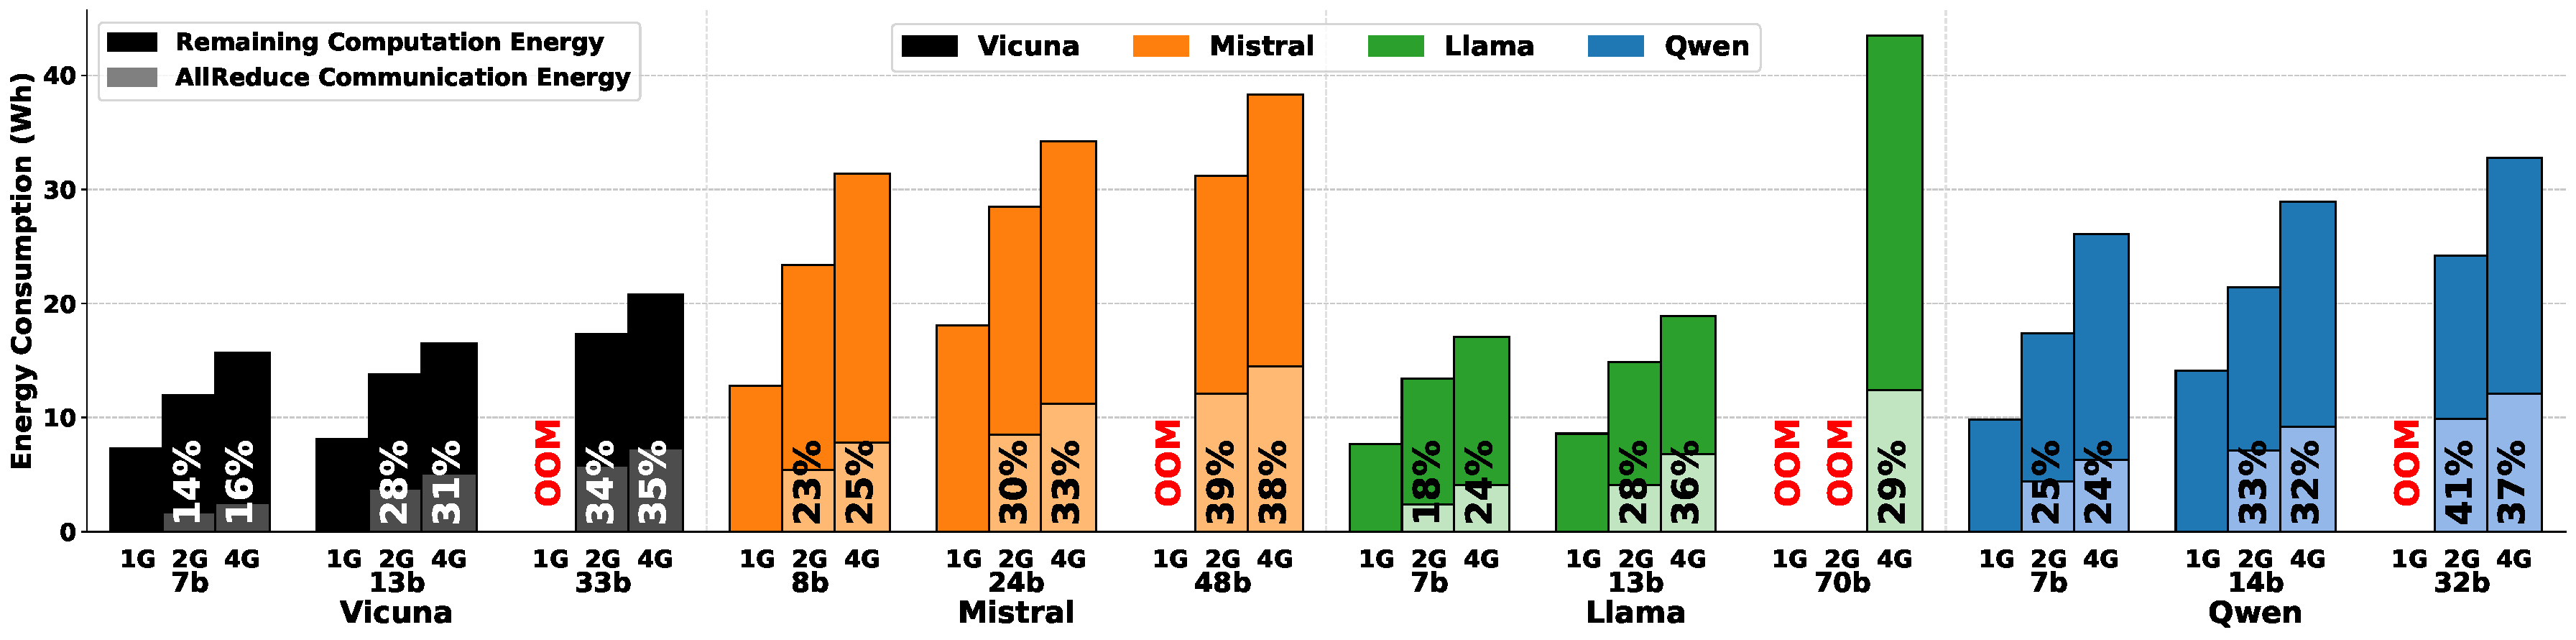
\includegraphics[width=\textwidth]{figures/llm_energy_comparison.pdf}
    \vspace{-24pt}
    \caption{Energy consumption across models and GPU configurations (2- and 4-GPU runs use tensor parallelism). Bars show total model energy; lighter segments show AllReduce communication energy (\% shown) and darker segments show remaining computation energy. Missing bars denote cases where model did not fit in GPU memory.} 
    \vspace{-15pt}
    \label{fig:all_reduce_energy}
\end{figure*}

%Our goal is to develop a methodology for predicting the energy consumption of parallel LLM inference over multiple GPUs.
There are three main parallelism strategies that are widely used for LLM inference, described below in increasing order of complexity.
%%%(see Appendices~\ref{app:collective-background} and \ref{app:data-collection-parallel} for more details).
\begin{enumerate}[leftmargin=*,itemsep=0pt,topsep=0pt]
    \item \textbf{Data parallelism} replicates the entire LLM on multiple GPUs, allowing input data to be processed in parallel~\cite{data-parallel}.
    \item \textbf{Pipeline parallelism} partitions the LLM into $s$ sequential stages, assigning each stage to a different GPU and processing micro-batches in a pipeline~\cite{sangjin23_envpipe}. 
    \item \textbf{Tensor parallelism} splits individual model computations (such as matrix multiplications) across multiple GPUs to enable parallel execution of operations~\cite{megatron}.
\end{enumerate}

\review{Tensor, pipeline, and data parallelism expose distinct communication patterns. In tensor parallelism, GPUs jointly execute operations within a layer, so partial results must be exchanged and combined using collectives such as AllReduce. Because these collectives occur repeatedly throughout the forward pass, communication is closely coupled with computation and synchronization.}

\review{Pipeline parallelism partitions layers across stages, and each stage sends its output activations to the next stage using point-to-point communication. Communication therefore occurs primarily at stage boundaries as activations move through the pipeline.}

\review{In data parallelism, each replica independently executes the full model on a different portion of the workload. Communication is therefore limited during the forward computation, with collective operations such as AllGather used when outputs from multiple replicas need to be consolidated.}

%Our framework can be extended to other strategies such as hybrid parallelism that combines existing parallelism methods; we leave this to future work.
%\medskip
%\subsection*{Challenges in predicting parallel inference energy}

There are two key challenges in accurately predicting the energy of parallel inference strategies.

\noindent\textbf{Compute energy.}
Even in single-GPU inference, compute energy depends on how \emph{each module}'s operator mix maps to GPU execution (e.g., memory behavior), which varies with tensor shapes and hardware/resource characteristics. 
%The energy traces for 10,000 individual Vicuna inference runs, collected on a NVIDIA A6000 GPU, are visibly noisy as well, as seen in(Figure~\ref{fig:energy-variance}).
%\anshul{need more details about the experiment, like which model and maybe point to S5x for experimental setup details. also, this figure should maybe go in non-determinism para, like the last para in this section?}
%\anurag{This is a single-GPU experiment, putting it in communication section seems improper as there is no communication here.}
%As a result, accurate modeling requires \emph{module-level} predictors that condition on both architecture-derived and resource/runtime features rather than a single aggregate utilization signal. 
In multi-GPU inference, this is further complicated because each module's computation and data may be divided across GPUs, so the model has to account for the energy consumption of the module at each GPU.
%%module computation is \be{sharded} across devices, so predicting a module's compute energy requires accounting for the per-rank shard (its local tensor shapes and execution) and then composing these shard-level estimates into an end-to-end module-level energy estimate. \aruna{I dont think I quite understand what this challenge is and how we solve it}

% Even in single-GPU inference, compute energy is difficult to predict because it is not a simple analytical function of token counts or average utilization. Instead, it depends on how the model’s operator mix maps to GPU execution at a fine granularity: different layers alternate between compute- and memory-bound phases, exhibit different cache reuse and memory-traffic patterns, and trigger different kernel schedules and concurrency across SMs.
% These effects make energy sensitive to seemingly small changes in tensor shapes (e.g., batch size, prefill vs.\ decode, and sequence-length-dependent activation sizes), and to runtime dynamics such as kernel launch ordering and power-state behavior under bursty workloads.
% In multi-GPU inference, these compute-side sensitivities persist on each GPU, but become more consequential because small per-GPU compute fluctuations can create \emph{stragglers} that change when synchronization points are reached, thereby affecting end-to-end energy beyond the local compute cost.
% \anurag{Make the compute energy smaller}

\noindent\textbf{Communication energy.}
\review{Multi-GPU inference additionally incurs \emph{substantial} energy from inter-GPU communication, including AllReduce in tensor parallelism, point-to-point transfers in pipeline parallelism, and AllGather in data parallelism, which is absent in single-device execution.}
% \noindent\textbf{Communication energy.}
% Multi-GPU inference additionally incurs \emph{substantial} energy from inter-GPU communication (e.g., AllReduce/ReduceScatter/AllGather, see Appendix~\ref{app:collective-background}), 
%\aruna{if you define these somewhere in the appendix, please add a reference}, 
% which is absent in single-device execution.
%and can form a large fraction of end-to-end energy. 
Figure~\ref{fig:all_reduce_energy} shows the measured energy consumption for 4 different LLM models under different GPU settings;
%(some larger models run out of memory when run with limited parallelization). 
details of the setup can be found in \S\ref{s:evaluation}. 
 Communication energy accounts for a large fraction (up to 41\%) of the total energy consumption.
%is due to communication energy, denoted as lighter segments in the figure.
% \be{Predicting communication energy is challenging} because communication is not a standalone phase: in tensor parallelism, collectives are frequently \emph{interleaved with} and \emph{overlapped with} computation for efficiency, so the measured energy reflects a mixture of compute, data movement, and synchronization overhead.
%%As such, communication modules must be \emph{accounted for explicitly} in the model tree; ignoring them leads to large prediction errors (see \S\ref{sec:ablation}).
%Accurately measuring this component is challenging as it requires tracking each of the numerous communication events on each GPU.
Tensor parallelism specifically introduces additional variance in energy consumption as
GPUs may lag/lead each other non-deterministically.
%but because they have to synchronize with each other frequently, the total energy consumption is non-deterministic. 

%This introduces additional complications due \be{synchronization induced non-determinism} %that directly perturbs communication energy across runs.
%collective-related GPU/NIC buffer activity begins and when transfer completes across the cluster, and then benchmarking these collectives under the target GPU count and topology to obtain representative energy costs that can be composed with module-level compute predictions.
% \anurag{I am sure we definitely do this and the design section will reflect this}
%\arunacomment{This last sentence sounds complicated and it is not clear to me how we are addressing this.}
%\anshul{I simplified the last sentence a bit, check. this says why direct measurement of comm energy is challenging}
%\begin{figure}[t]
    % \centering
 %   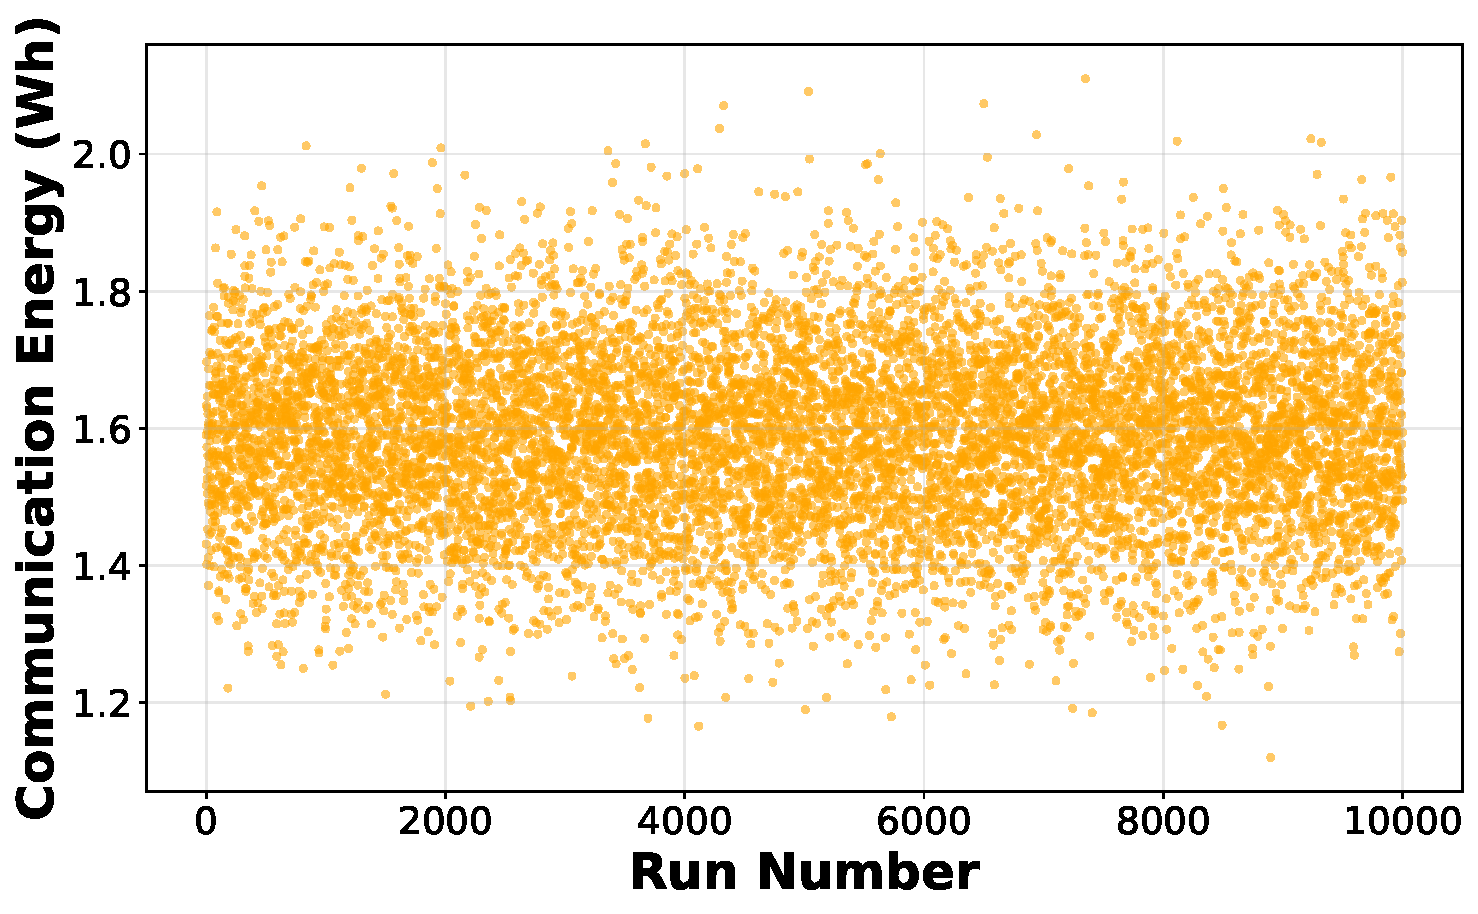
\includegraphics[width=0.48\textwidth]{figures/comm-energy-vs-run.pdf}
 %   \caption{Communication energy consumption for 10,000 Vicuna-7b tensor-parallel inference runs (128 output tokens) on 4 NVIDIA A6000 GPUs.}
  %  \label{fig:energy-variance}
%\end{figure}

%\noindent\textbf{Non-determinism.}
%\aruna{If we remove the figure, will this whole non-determinism piece go away? or do we still something about the non-determinism}
%Beyond this measurement complexity, tensor parallelism specifically introduces additional challenges with \be{synchronization} across GPUs as the ReduceScatter/AllGather phase is interleaved with layer computation for high efficiency.
%This introduces additional complications due \be{synchronization induced non-determinism} %that directly perturbs communication energy across runs.
%GPUs may lag/lead each other \be{non-deterministically} due to compute-time variation (e.g., memory-access and caching effects, hardware scheduling), creating \emph{idle-but-powered} intervals whose duration depends on runtime contention and race conditions. 
%Consequently, the time spent and the energy consumed in the communication phases can change even under \emph{identical} inputs and configurations.
%As shown in Figure~\ref{fig:energy-variance}, significant variation is observed in the measured communication energy when the same tensor-parallel inference (Vicuna-7b, in this case) is executed multiple times; see Section~\ref{ss:esetup} for experimental setup details.
%This creates \emph{idle-but-powered} intervals whose duration depends on runtime contention and race conditions. 
%This makes energy prediction more challenging. % complicating both isolating ``pure transfer'' energy from waiting energy and predicting a stable communication-energy contribution rather than a single deterministic trace.


% LLM energy consumption under parallel inference is driven by not only the computation cost, but also the \be{inter-GPU communication costs}. 
% This matters because communication can be a large fraction of total energy: Figure~\ref{fig:all_reduce_energy} shows that, for tensor-parallel runs, collective communication (e.g., AllReduce) contributes a substantial portion of end-to-end energy across model families and GPU counts (e.g., 14.2\%--35.1\% for Vicuna as model and GPU count scale). 
% \review{
% Predictors that extrapolate energy to multi-GPU settings solely from compute (or from per-rank tensor operations) systematically miss this component and can incur large errors.
% \textbf{Compute energy itself is non-trivial to model}, since it depends on how kernels exercise GPU resources (SM activity, memory intensity, and power-state behavior) across heterogeneous LLM modules.
% Prior work often sidesteps this by using \emph{coarse power measurements} (e.g., NVML board power sampled over time) or workload-level estimators (e.g., Strubell et al.’s energy-as-power$\times$time style accounting), and systems such as IrEne build learned predictors from profiled execution statistics.
% However, these approaches are typically \emph{coarse-grained and single-GPU oriented}, and they do not directly support accurate \emph{module-level} attribution under overlapping compute/communication in multi-GPU inference.
% }
% The severity and predictability of communication overhead differs across parallelism strategies.
% Under data parallelism, the replicas work independently,  
% except for the collation of output from each replica in the AllGather phase; as such, the additional energy of this phase needs to be accounted for. 
% %The AllGather phase is largely deterministic, so predicting the energy consumption under data parallel inference is feasible. 
% For pipeline parallelism, we have to track the energy consumption when data is sent from one stage to the other, in addition to the local computation. These data transfers happen in sync with each stage's computations and the timing can vary depending on sequence length and network speeds.

% Tensor parallelism is the most challenging of the three cases because synchronization across GPUs (e.g., ReduceScatter/AllGather) is interleaved with layer computation for high efficiency. This leads to two main challenges: 

% \noindent (i) \be{Non-determinism} in GPU wait times as GPUs often lag/lead each other in compute operations (due to variations in memory access, caching effects, hardware scheduling) during the synchronization phase. 
% From a measurement standpoint, this causes difficulty in isolating AllReduce energy as it requires distinguishing between the non-deterministic waiting phase (where GPUs are idle) and the network transfer phase.

% \noindent (ii) \be{Fine-grained energy accounting} is challenging as AllReduce overlaps computation and network transfer. 
% From a prediction standpoint, this requires isolating the different sources of energy consumption and accounting for them. 
% This is not an issue in pipeline and data parallelism as GPU communication and computation are not synchronized. 
% \review{
% Finally, \sys{} must also generalize across heterogeneous LLM variants, architectures, and deployment configurations, since changes in block structure (e.g., attention/MLP variants) and parallelization degree alter tensor shapes and collective-communication patterns, making predictors calibrated on one model/config unreliable on another~\cite{ultima}.
% }
%\smallskip\noindent{\textbf{Challenges: Communication energy in parallel inference.}}
%Energy consumption under parallel inference is shaped not only by local computation but also by inter-GPU \emph{communication} and the synchronization it induces. 
%}


\section{Design of \sys{}}
\label{s:piep}
Figure~\ref{fig:piep_architecture} presents an overview of the \sys{} architecture. \sys{}
first decomposes the LLM into individual constituent modules (\S\ref{ss:design-decomposition}), allowing \sys{} to directly model the energy consumption of compute and communication in parallel inference.
Since the number of GPUs involved in parallel inference influences the energy consumption and tensor shapes of individual modules, \sys{} makes use of resource- and architecture-aware features for each module based on the parallelization strategy (\S\ref{ss:design-features}).
\sys{} then explicitly predicts the energy used for GPU communication (\S\ref{ss:design-communication}) and carefully measures both computation and communication energy to collect ground truth (\S\ref{ss:design-measurement}).
Finally, \sys{} builds a multi-level regressor to combine these contributions to accurately learn end-to-end energy (\S\ref{ss:design-prediction}).

\begin{figure*}[t]
\centering
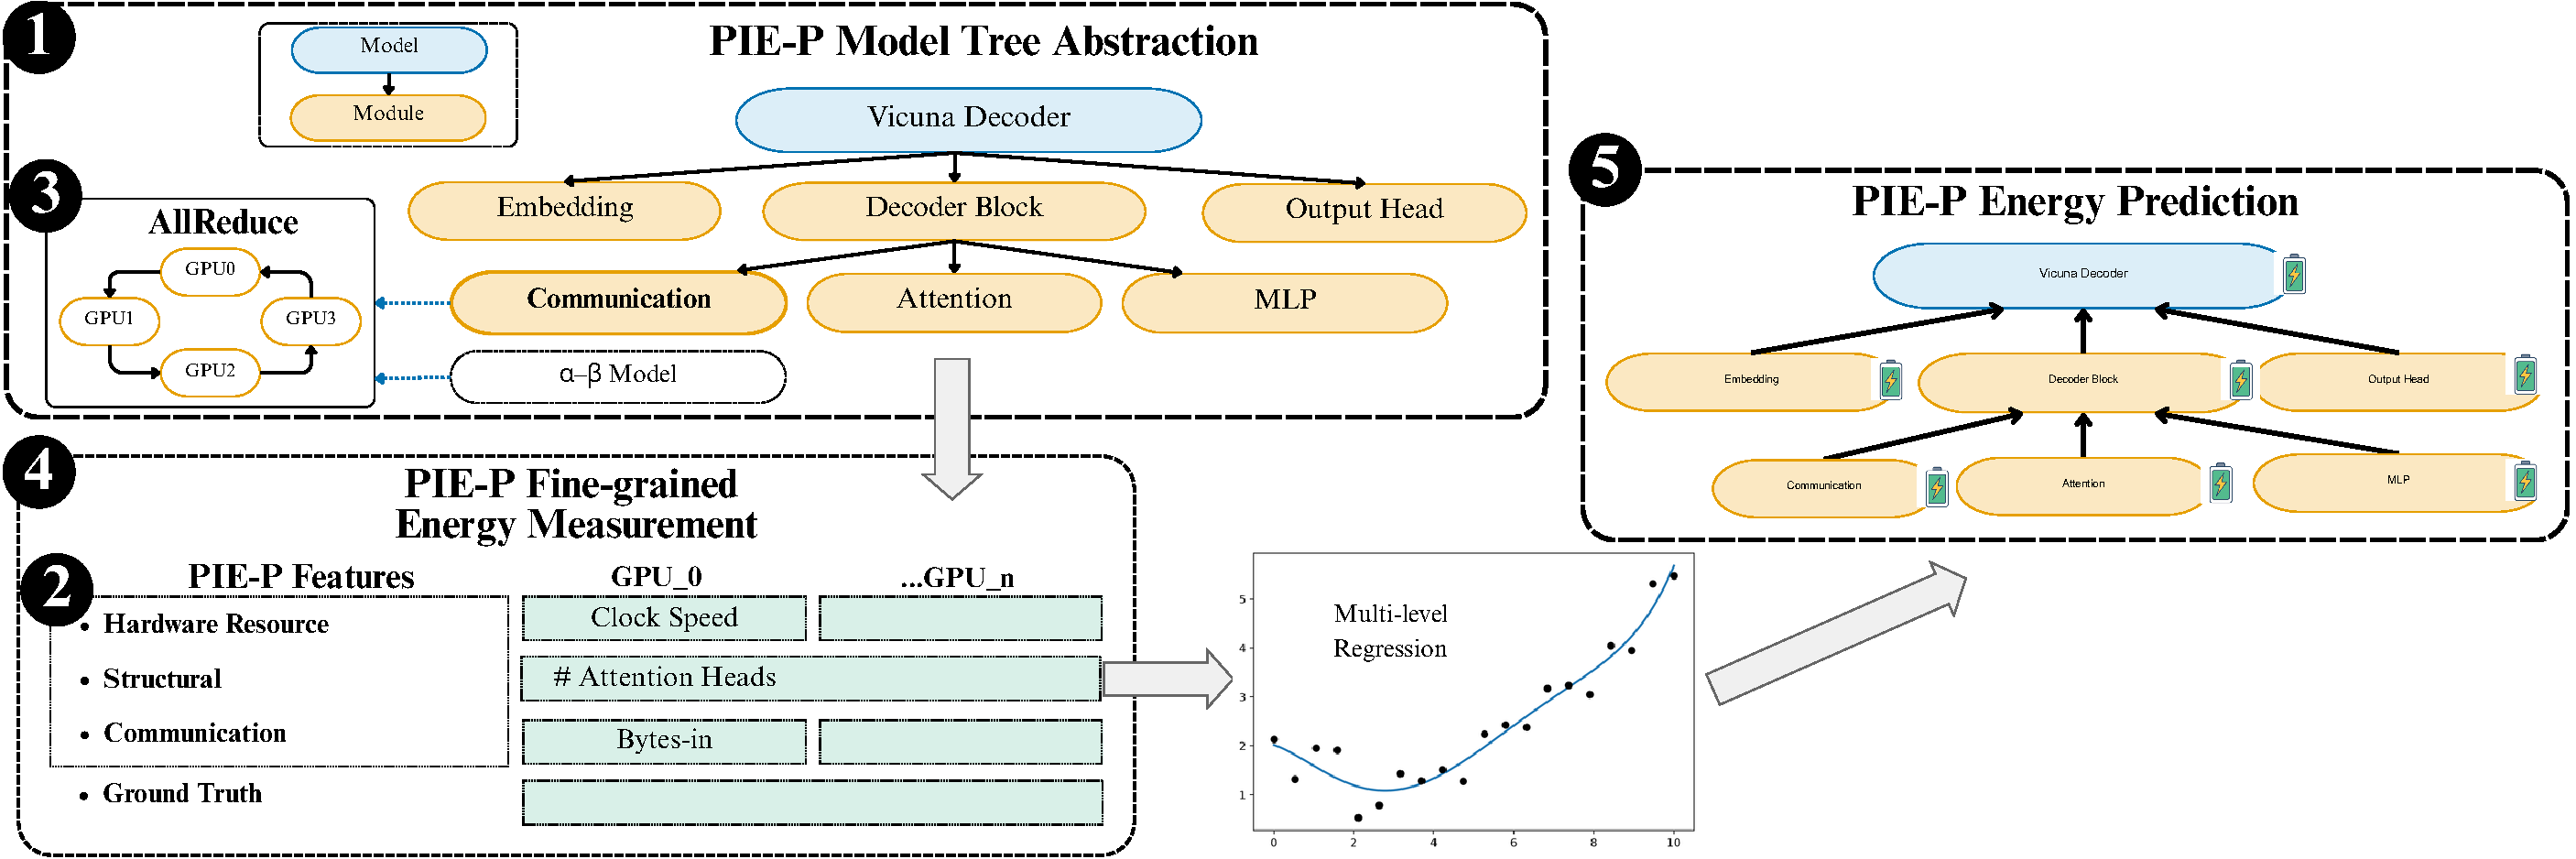
\includegraphics[
    width=\textwidth,
    height=0.20\textheight,
    keepaspectratio
]{figures/piepv6.pdf}
\vspace{-9pt}
\caption{\sys{} architecture showing: (1) parallelism-aware decomposition, (2) features for module-level prediction, (3) communication energy modeling, (4) measurement and data collection, and (5) multi-level regression.}
\label{fig:piep_architecture}
\vspace{-18pt}
\end{figure*}

\subsection{Parallelism-Aware Decomposition into Compute and Communication Modules}
\label{ss:design-decomposition}

\sys{} uses a \emph{model-tree abstraction}, a graph-structured representation to decompose the inference run into constituent units (i.e., modules). Unlike prior work (e.g., IrEne~\cite{irene}) that only focuses on compute modules, the \sys{} model tree decomposes a model using both compute \emph{and} communication modules.

Concretely, \sys{} represents an LLM inference run as a hierarchical composition of modules, where each Transformer block is decomposed into child modules (e.g., AllReduce, Attention, MLP, normalization, embedding, output).
For inter-GPU communication, such as AllReduce operations, \sys{} adds a separate communication module to the model tree and records the data transferred between GPUs (see Figure~\ref{fig:piep_architecture}); this is then used to predict communication energy as discussed in \S\ref{ss:design-communication}.
This decomposition into modules can be obtained from existing ML frameworks, including PyTorch (using \texttt{torch.fx} symbolic tracing) or TensorFlow (using graph tracing).

\subsection{Features for Module-Level Prediction}
\label{ss:design-features}

To capture the relationship between energy and the compute and communication modules, \sys{} leverages hardware resource, model execution, and model structural features.
For example, the \emph{number of attention heads} influences how work is divided across GPUs during tensor parallelization, affecting communication volume in AllReduce operations.
We thus extract such structural features from the model for parallelized energy prediction; existing utilization- or metrics-based heuristics~\cite{strubell19,Nguyen-hotcarbon,wilkins2024offlineenergyoptimalllmserving} miss out on this critical information.

\begin{table}[t]
\centering
\small
\setlength{\tabcolsep}{4pt}
\renewcommand{\arraystretch}{1.05}
\begin{tabular}{@{}
>{\raggedright\arraybackslash}p{0.48\linewidth}
>{\raggedright\arraybackslash}p{0.48\linewidth}
@{}}
\toprule
\rowcolor{rowblue}
\multicolumn{2}{@{}l@{}}{\textbf{Resource Utilization Features}}\\
\midrule
CPU utilization (\%) & CPU mem. utilization (\%)\\
\rowcolor{rowblue} GPU utilization (\%) & GPU mem. utilization (\%)\\
CPU clock (GHz) & CPU mem. clock (GHz)\\
\rowcolor{rowblue} Memory (bytes) & GPU clock (GHz)\\
GPU mem. clock (GHz) & \\
\midrule
\rowcolor{rowblue}
\multicolumn{2}{@{}l@{}}{\textbf{Execution Features}}\\
\midrule
Batch size & Sequence length\\
\rowcolor{rowblue} FLOPs per token (billions) & Execution time (s)\\
GPU energy NVML (Wh) & Number of GPUs\\
\midrule
\rowcolor{rowblue}
\multicolumn{2}{@{}l@{}}{\textbf{Model Structure Features}}\\
\midrule
Feed-forward dimension & Transformer blocks\\
\rowcolor{rowblue} Hidden embedding size & Attention heads\\
Key--value heads & \\
\midrule
\rowcolor{rowblue}
\multicolumn{2}{@{}l@{}}{\textbf{Communication Features}}\\
\midrule
Bytes transferred & Effective bandwidth\\
\bottomrule
\end{tabular}
\caption{Features used by \sys{} for prediction.}
\label{tab:features}
\end{table}

Table~\ref{tab:features} summarizes the complete feature set.
Resource utilization features capture system- and device-level activity during inference; execution features capture the workload configuration that drives runtime and energy; and model-structure features capture architectural properties that determine tensor sizes.
For communication modules, \sys{} additionally uses the amount of data transferred and the effective bandwidth of each inter-GPU communication event.
A Spearman analysis across Vicuna configurations further shows that total energy correlates not only with NVML GPU energy ($\rho=0.633$--$0.762$), but also with batch size ($\rho=0.735$--$0.737$), execution time ($\rho=0.658$--$0.664$), and memory usage ($\rho=0.656$--$0.663$), motivating the use of multiple runtime and structural features rather than a single utilization signal.

\subsection{Communication Energy Modeling}
\label{ss:design-communication}

To model the communication energy introduced by parallel inference, \sys{} first treats inter-GPU communication events as explicit modules in the model tree.
For each communication event $e$, we trace the communication tensor sizes and calculate network transfer bytes sent ($B_{e}^{\mathrm{out}}$) and received ($B_{e}^{\mathrm{in}}$) by each GPU and use an offline-calibrated $\alpha$--$\beta$ model~\cite{hockney1988parallel2} to estimate the communication latency as:

\vspace{-12pt}
\begin{equation}
\label{eq:comm-latency-main}
T_{e}^{\mathrm{comm}} =
\alpha_{o,p} +
\beta_{o,p}
\left(
B_{e}^{\mathrm{out}} + B_{e}^{\mathrm{in}}
\right),
\end{equation}
\vspace{-8pt}
where $o$ denotes the communication operation (e.g., AllReduce or point-to-point transfer), $p$ is the number of GPUs, $\alpha_{o,p}$ captures the fixed communication overhead, and $\beta_{o,p}$ captures the message-size-dependent transfer cost.
For each event, we define the per-GPU communication volume as $V_e=B_e^{\mathrm{out}}+B_e^{\mathrm{in}}$.

We calibrate $\alpha_{o,p}$ and $\beta_{o,p}$ offline for each communication operation and GPU count by recording the observed communication time and volume across calibration runs and fitting $T_e^{\mathrm{obs}}=\alpha_{o,p}+\beta_{o,p}V_e$.
The corresponding effective bandwidth is $B^{\mathrm{eff}}_{o,p}=1/\beta_{o,p}$.
For ring AllReduce, a tensor of size $S_e$ bytes results in a per-GPU communication volume of
\begin{equation}
V_e^{\mathrm{AR}} = \frac{2(p-1)}{p}S_e,
\label{eq:allreduce_volume}
\end{equation}
accounting for both the ReduceScatter and AllGather phases.
For pipeline-parallel point-to-point transfers and data-parallel AllGather operations, we compute the communication volume from the transferred tensor size using the corresponding communication pattern.

Finally, \sys{} converts the predicted communication latency to communication-module energy by multiplying it with the calibrated average communication power $\bar{P}^{\mathrm{comm}}_{o,p}$:
\begin{equation}
\widehat{E}^{\mathrm{comm}}_e =
\bar{P}^{\mathrm{comm}}_{o,p} T_e^{\mathrm{comm}}.
\label{eq:comm_energy}
\end{equation}
The resulting communication-module estimate is then composed with the compute-module estimates by the multi-level regressor described in \S\ref{ss:design-prediction}.

\subsection{Measurement and Data Collection}
\label{ss:design-measurement}

\sys{} measures communication energy by first identifying the communication events introduced by each parallelism strategy and then isolating the corresponding windows in the execution trace. We align these communication windows with the system power trace and integrate power over the corresponding intervals to obtain communication-energy measurements for training the communication-module predictor. Effective bandwidth is computed from the observed communication volume and transfer time, while bytes sent and received are derived from the tensor size being communicated.

The communication window is identified differently for each parallelism strategy. \textbf{Tensor parallelism:} we profile ring AllReduce repeatedly to capture the distribution of synchronization and communication energy caused by non-deterministic leading and lagging GPU behavior. The profiled window includes both hop transfers and synchronization stalls across the ReduceScatter and AllGather phases. \textbf{Pipeline parallelism:} for each stage boundary, we use \texttt{nsys} to timestamp the end of stage $i$'s last forward kernel and the start of stage $i{+}1$'s first forward kernel; the intervening interval is attributed to the point-to-point activation transfer, and power is integrated over this window. \textbf{Data parallelism:} replicas execute their local forward passes independently and perform a tail-end AllGather to collate final outputs; we profile this final output stage to measure the corresponding communication energy.

For compute modules, \sys{} records (i) resource-specific signals that summarize system/GPU activity and (ii) model-specific descriptors extracted from the LLM configuration.
\sys{} collects repeated offline measurements for each module across controlled execution runs to build a stable training dataset for the module-level regressors (\S\ref{ss:design-prediction}). This captures non-deterministic straggler effects in observed communication behavior and improves the stability of the learned regressors. Because all profiling and calibration are performed offline, \sys{} incurs no additional measurement overhead during inference.

\subsection{Multi-Level Regression}
\label{ss:design-prediction}

Our methodology for training regressors follows a hierarchical approach, training module-level predictors and then combining them for model-level prediction.
As \sys{} obtains features from multiple GPUs, naively learning separate coefficients per GPU does not scale as the number of parameters grows with GPU count.
Instead, \sys{} computes statistical aggregates of runtime features using the mean, standard deviation, minimum, and maximum across all GPUs. These are combined with the static structural features to form the complete feature vector for each sample.

\sys{} uses the following multi-level regression formulation:
\vspace{-6pt}
\begin{equation}
\small
\begin{aligned}
P_e(m) &=
\sum_{c \in \mathcal{C}(m)} \alpha(c)\,P_e(c),\\[2pt]
P_e(c) &=
f_{\mathrm{Module}(c)}\!\left(\mathrm{feat}(c)\right)
\quad \text{if } c \text{ is a compute module},\\[2pt]
P_e(c) &=
\bar{P}^{\mathrm{comm}}_{o(c),p}\,
T_{c}^{\mathrm{comm}}
\quad \text{if } c \text{ is a communication module},\\[3pt]
\alpha(c) &=
1 + \frac{\tanh(\mathbf{W}\,\mathrm{feat}(c)+b)}{\tau}.
\end{aligned}
\label{eqn:end2end-predicted-sum}
\vspace{-7pt}
\end{equation}

Eq.~(\ref{eqn:end2end-predicted-sum}) defines the final model-level prediction. Here, $P_e(m)$ denotes the predicted end-to-end energy of model $m$, and $\mathcal{C}(m)$ is the set of compute and communication modules.
For a compute module $c$, $P_e(c)$ is predicted using the module-specific regression function $f_{\mathrm{Module}(c)}$; in our implementation, this is a decision-tree regressor trained separately for each module type.
For a communication module $c$, $P_e(c)$ is computed as the average observed communication power $\bar{P}^{\mathrm{comm}}_{o(c),p}$ multiplied by the communication time $T_{c}^{\mathrm{comm}}$ obtained from Eq.~\eqref{eq:comm-latency-main}. The average communication power is calibrated for communication operation type $o(c)$ (e.g., AllReduce, AllGather) and GPU count $p$.
Finally, $\alpha(c)$ is the learned composition weight for module $c$.
This formulation makes the bottom-up prediction explicit: \sys{} first predicts the energy of compute and communication modules, then combines those module-level predictions to obtain the model-level energy $P_e(m)$.

This hierarchical composition enables \emph{cross-variant and cross-model reuse} since many modules (e.g., Attention and MLP blocks) are shared across different models. While we do not claim generalization to arbitrary architectures, our results in \S\ref{sec:model_prediction} demonstrate that \sys{} generalizes across multiple model families.


\section{Evaluation}
\label{s:evaluation}
\begin{figure*}[!ht]
    \centering
    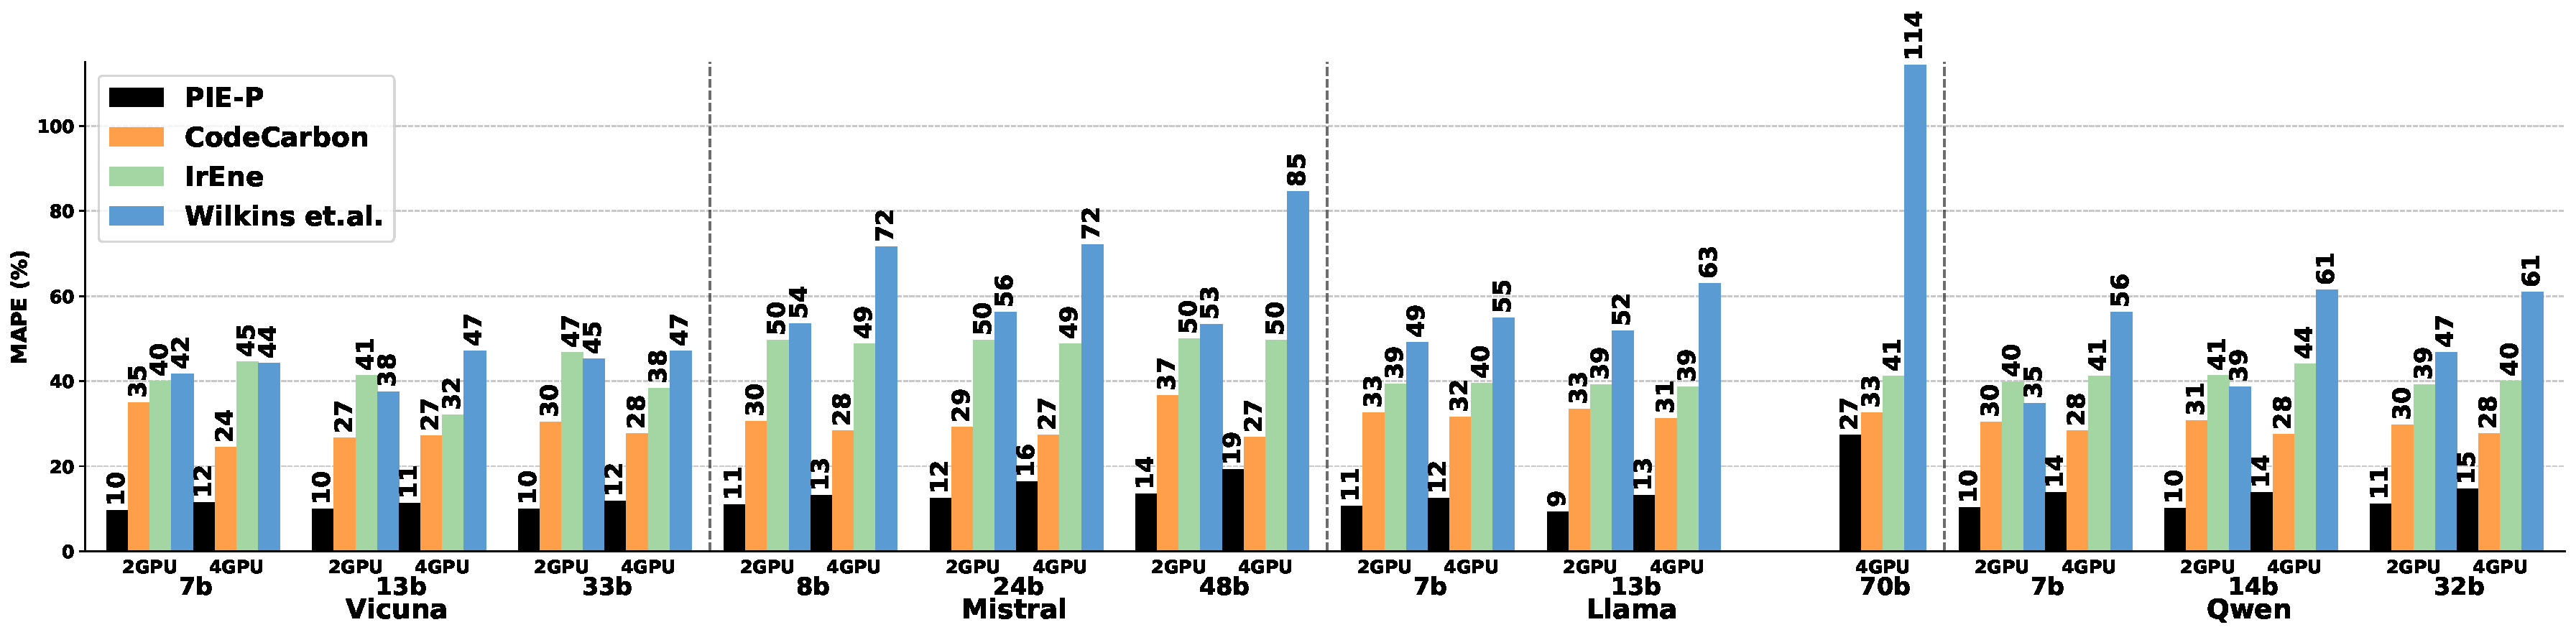
\includegraphics[width=\textwidth]{figures/mape_all_model_families.pdf}
    \vspace{-24pt}
    \caption{MAPE results across model families for \sys{} and the baselines under tensor parallelism on A6000.}
    \label{fig:mape_comparison}
    \vspace{-9pt}
\end{figure*}

\begin{figure*}[!t]
\centering
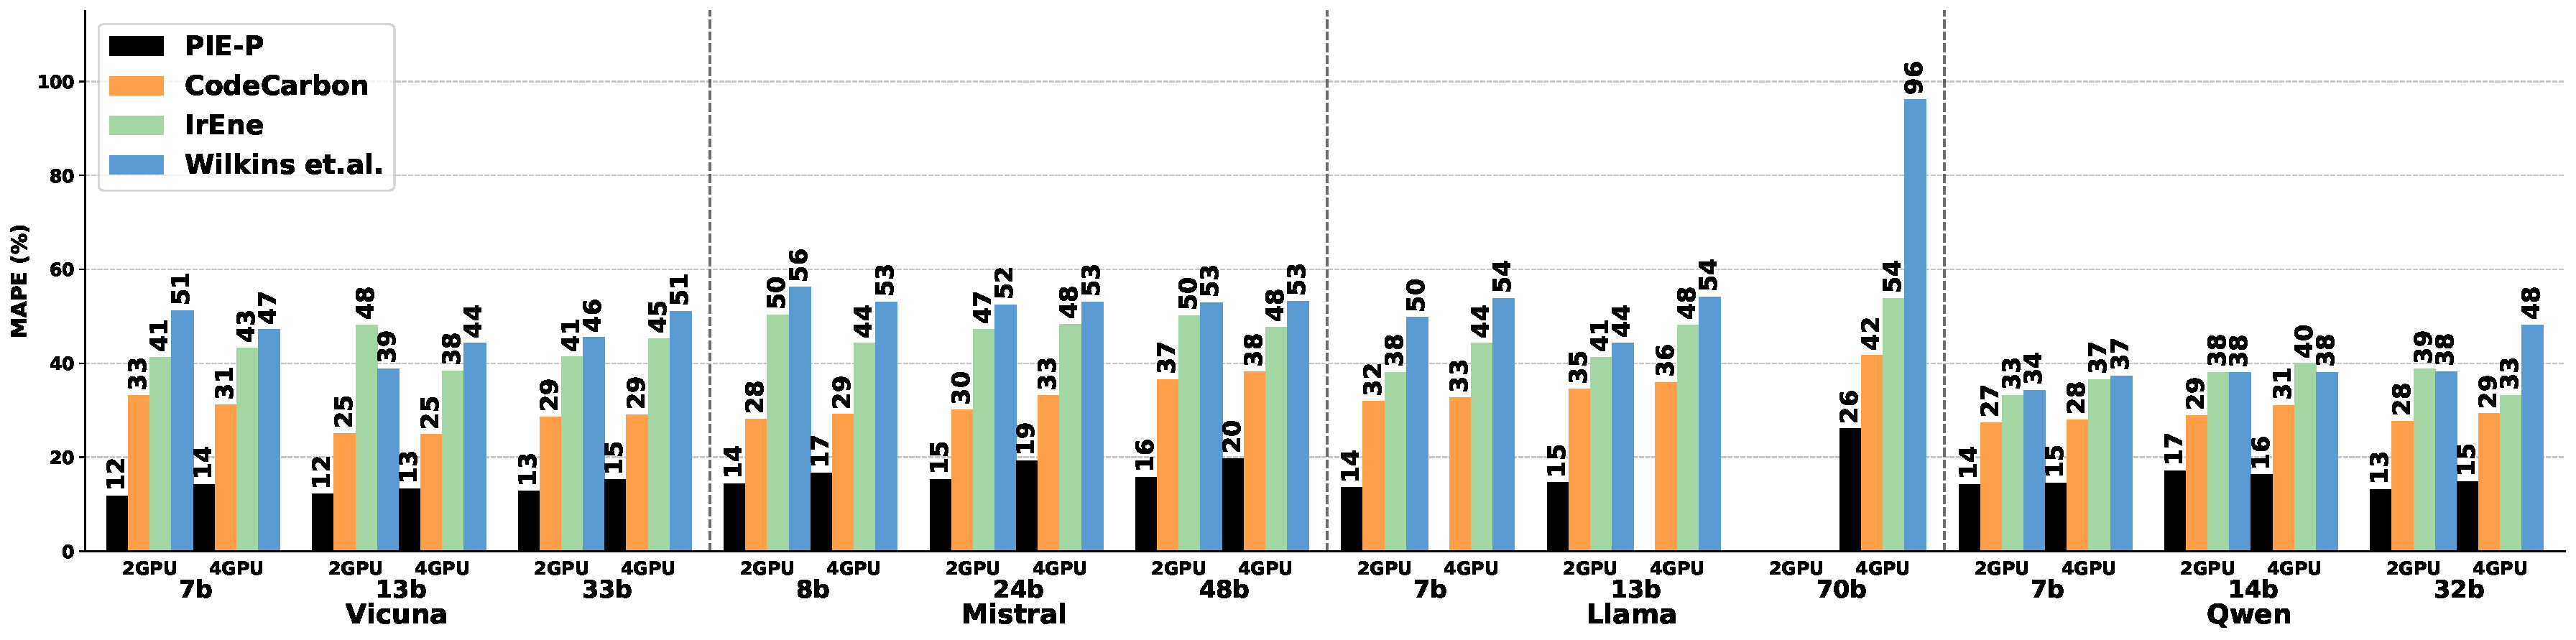
\includegraphics[width=\textwidth]{figures/b40_mape_tensor_parallelism_with_codecarbon.pdf}
\vspace{-24pt}
\caption{MAPE results across model families for \sys{} and the baselines under tensor parallelism on B40.}
\label{fig:b40_mape_tensor_parallelism}
\vspace{-18pt}
\end{figure*}

Our evaluation demonstrates \sys{}'s effectiveness across four LLM model families across varying sizes (7B--70B): Vicuna, Mistral, Llama, and Qwen~\cite{vicuna, jiang2023mistral7b, touvron2023llama, qwen}.
We experiment on three different hardware platforms that use different communication modes (NVLink and PCIe) across the three widely employed parallelization strategies (tensor, pipeline, and data). We evaluate all three forms of parallelism, while using tensor parallelism for the most extensive analysis because individual model operators are partitioned across GPUs and collective communication is repeatedly interleaved with computation inside Transformer blocks. This makes its communication and synchronization behavior substantially more involved than the stage-boundary transfers in pipeline parallelism and the less frequent communication in our data-parallel inference setup.

\subsection{Evaluation Methodology}
\label{ss:esetup}
We conducted experiments on three hardware platforms:
(1) NVIDIA RTX A6000;
(2) NVIDIA B40; and
(3) NVIDIA H200.
Platform (1) uses an AMD EPYC Milan 7543P 32-core CPU with four A6000 GPUs over PCIe 4.0. Platforms (2) and (3) use an Intel Xeon 6 6530P 32-core CPU with PCIe 4.0 for B40 and NVLink-connected GPUs for H200.
Ground-truth system power/energy is measured using an external Watts Up Pro monitor (platform~1) and IPMI/BMC power readings (platforms 2,3).

\anurag{Appendix - E Methodology: Training}
\review{\smallskip\noindent\textbf{Training methodology.} We train \sys{} hierarchically: module-level predictors are learned first and their predictions are then composed into model-level energy. We use 3-fold cross-validation at the module level with a 70\%/30\% train/test split. Each module type (e.g., Self-Attention, MLP, and AllReduce) is sampled $10{,}000$ times to build a robust dataset. A sample is an aggregate measurement formed by running the module $100{,}000$ times under a fixed model and GPU configuration. For every sample, runtime features across the participating GPUs are reduced to their mean, standard deviation, minimum, and maximum values to capture both the overall activity level and cross-GPU imbalance, and these statistics are combined with the structural features in Table~\ref{tab:features}.}

\review{To expose the predictors to different operating regimes, we profile batch sizes 8, 16, 32, and 64 and output sequence lengths 512 and 1024. We use DeepSpeed~\cite{deepspeed} for tensor-, pipeline-, and data-parallel inference. We evaluate generalization using leave-one-out experiments because a useful predictor should transfer to models that were not present in its training measurements. In leave-one-variant-out evaluation, an entire model variant is excluded and predicted using module-level predictors learned from the remaining variants in the same family. In leave-one-family-out evaluation, all variants of one family are excluded from training, providing a stricter test of transfer across model architectures.}

\review{Our primary tensor-parallel evaluation covers the complete model suite on the A6000 and B40 platforms. We then use representative experiments on the H200 and in the additional generalization analyses to test whether the same decomposition and feature design continue to work across different hardware and model settings. We do not repeat every experiment on every model--hardware combination; instead, the full suite establishes the main result and the representative experiments test the relevant generalization dimensions.}

\smallskip\noindent\textbf{Baselines and comparison variants.} We compare \sys{} against the following prediction and measurement baselines, together with controlled variants that isolate the contribution of its design choices. \\
\noindent\textbf{\be{IrEne}~\cite{irene}:} A hierarchical energy prediction framework for single-GPU execution and the closest methodological baseline to \sys{}. IrEne represents execution at mathematical-operation, machine-learning-operation, and module levels, learns leaf-level energy predictors from runtime resource utilization and model specifications, and recursively combines child predictions to obtain higher-level energy estimates. We use IrEne in the same inference configurations as \sys{}; its key limitation for our setting is that the hierarchy does not represent inter-GPU communication as a first-class module. \\
\textbf{\be{CodeCarbon}~\cite{codecarbon}:} A software-based energy/\(\mathrm{CO_2}\) estimator that integrates telemetry-derived power over time, including GPU measurements from NVML and host measurements where available. It provides a commonly used software-only estimate, but does not explicitly represent the communication structure introduced by parallel inference. \\
\textbf{\be{Wilkins et al.}~\cite{wilkins2024offlineenergyoptimalllmserving}:} A per-request energy predictor based on prompt and output lengths. We implement the token-in/token-out model by fitting $e_K(\tau_{\mathrm{in}},\tau_{\mathrm{out}})=\alpha_0\tau_{\mathrm{in}}+\alpha_1\tau_{\mathrm{out}}+\alpha_2\tau_{\mathrm{in}}\tau_{\mathrm{out}}$ on a calibration set. \\
\textbf{\be{NVML}~\cite{nvml}:} A widely used software source of GPU power/energy telemetry~\cite{strubell19,luccioni2022estimatingcarbonfootprintbloom,Jesse-dodge-icml}. To test whether GPU-only energy is sufficient to predict full-system energy, we train a model-level linear regressor with NVML-reported GPU energy as the independent variable and the wall-meter/IPMI measurement as the prediction target. \\
\textbf{\be{\textsc{AvgComm}} (\sys{} without explicit communication modeling):} This variant retains the model-tree decomposition and compute-module predictors, but replaces \sys{}'s communication model with a simpler estimate that multiplies an average observed AllReduce power by the duration of each collective. It directly tests whether treating communication as a structured, volume- and topology-dependent module is necessary. \\
\textbf{\be{\sys{} without model-tree decomposition}:} We remove the module-level hierarchy and train a single model-level regressor from aggregate features. This comparison isolates whether fine-grained decomposition is needed beyond simply supplying the same broad classes of signals to one predictor. \\
\textbf{\be{NeuSight-style energy predictor}~\cite{neusight}:} We retain NeuSight's fine-grained matrix-tile decomposition, FLOP/memory features, and MLP prediction structure, but replace latency with measured system energy as the target. This tests whether a representation designed for latency prediction can be directly retargeted to energy.

We omit the software-based estimator of Strubell et al.~\cite{strubell19} as it is outperformed by baselines such as IrEne~\cite{irene}.

\review{\smallskip\noindent\textbf{Summary of results.} \sys{} maintains low prediction error across all three parallelization strategies. Tensor parallelism is the most demanding setting, yet \sys{} achieves average MAPE in the mid-teens on both A6000 and B40, with representative H200 results showing comparable behavior on an NVLink platform. The same framework achieves 12.2\% average MAPE for pipeline parallelism and 10.8\% for data parallelism. Module-level and leave-one-out results further show that the predictor transfers across model components, model sizes, model families, and hardware settings rather than only fitting individual measured configurations.}

\subsection{Energy Prediction for Tensor Parallelism}
\label{sec:model_prediction}
Figures~\ref{fig:mape_comparison} and~\ref{fig:b40_mape_tensor_parallelism} show the mean absolute percentage error (MAPE) for \sys{} and the baselines under tensor parallelism on A6000 and B40 GPUs, respectively.
For each model family (e.g., Vicuna), we train a regressor on 70\% of module-level predictions across all variants (e.g., 7B), batch sizes, and input lengths, and evaluate on the remaining 30\%, following the training protocol in \S\ref{ss:esetup}.

We see that \be{\sys{} consistently achieves the lowest MAPE in all cases} on the A6000 platform, with an average of 17.6\%.
By contrast, CodeCarbon incurs an average MAPE of 28.49\%, which is about 1.7$\times$ the MAPE of \sys{}.
The poor prediction of CodeCarbon is because of its reliance on coarse GPU profiling and slow sampling, which misses the energy use of fine-grained, multi-GPU communication events.
IrEne also performs poorly, with an average MAPE of 40.45\% (about 3$\times$ that of \sys{}) because it ignores communication energy.
Finally, Wilkins et al. consistently incurs high MAPE, with an average of 58.77\% (more than 4$\times$ that of \sys{}) because it solely uses a token-in/token-out regression that ignores inter-GPU communication.

The B40 results in Figure~\ref{fig:b40_mape_tensor_parallelism} show similar trends on a different GPU platform with \sys{} achieving an average MAPE of 15.5\%, substantially better than the other alternatives.
On closer inspection we observe that the \be{performance gap between \sys{} and the baselines widens with increasing parallelization}.
This is because the energy contribution of AllReduce, due to its ring communication, increases with the number of GPUs; see Figure~\ref{fig:all_reduce_energy}.

\anurag{Appendix - M Additional Results on NVIDIA H200 GPUs}
\review{We also evaluate \sys{} on 2$\times$ NVIDIA H200 GPUs to test whether the same model-tree decomposition, communication model, and feature set remain useful on a substantially different GPU/interconnect platform. Across the evaluated model variants, model-level MAPE averages 16.8\%, comparable to the A6000 and B40 experiments. Table~\ref{tab:h200_model_results} gives the per-variant results. The larger Llama-70B configuration is the most difficult at 26.53\%, while most other variants remain in the 13--19\% range.}

\begin{table}[t]
\centering
\small
\setlength{\tabcolsep}{5pt}
\renewcommand{\arraystretch}{1.05}
\begin{tabular}{lclc}
\toprule
\textbf{Model} & \textbf{MAPE} & \textbf{Model} & \textbf{MAPE} \\
\midrule
\rowcolor{rowblue} Vicuna 7B  & 13.34\% & Llama 7B  & 15.30\% \\
Vicuna 13B                    & 13.78\% & Llama 13B & 16.51\% \\
\rowcolor{rowblue} Vicuna 33B & 14.45\% & Llama 70B & 26.53\% \\
Mistral 8B                    & 16.25\% & Qwen 8B   & 16.07\% \\
\rowcolor{rowblue} Mistral 24B & 17.25\% & Qwen 14B  & 19.41\% \\
Mistral 48B                   & 17.83\% & Qwen 32B  & 14.90\% \\
\bottomrule
\end{tabular}
\caption{Model-level prediction results for \sys{} on 2$\times$ NVIDIA H200 GPUs.}
\label{tab:h200_model_results}
\end{table}

\review{The H200 module-level results in Table~\ref{tab:h200_module_results} are all single digit, including a 9.25\% MAPE for AllReduce. This provides evidence that the communication-aware component remains effective when moving from PCIe-oriented platforms to the H200's higher-bandwidth NVLink environment. We do not claim a hardware-agnostic predictor---\sys{} is still calibrated per platform---but the same decomposition and feature design are reused without modification.}

\begin{table}[t]
\centering
\small
\setlength{\tabcolsep}{6pt}
\renewcommand{\arraystretch}{1.05}
\begin{tabular}{lc}
\toprule
\textbf{Module} & \textbf{H200 MAPE} \\
\midrule
\rowcolor{rowblue} Self-Attention      & 8.80\% \\
MLP                                    & 7.44\% \\
\rowcolor{rowblue} AllReduce           & 9.25\% \\
LayerNorm/RMSNorm                      & 8.12\% \\
\rowcolor{rowblue} LLMEmbedding        & 7.78\% \\
\bottomrule
\end{tabular}
\caption{Module-level MAPE for \sys{} on NVIDIA H200 GPUs.}
\label{tab:h200_module_results}
\end{table}

\subsection{NVML Baseline Results}
\anurag{Appendix - G Additional results: NVML as a proxy for total energy}
\review{Table~\ref{tab:nvml_proxy_combined} reports the comparison with the NVML-based full-system energy regressor on A6000. In the direct setting, Vicuna ranges from 29.8--33.4\% MAPE, Mistral from 39.0--44.2\%, Llama from 28.5--31.3\%, and Qwen from 38.0--42.4\%. These errors are substantially larger than \sys{}, showing that GPU-board energy alone is not sufficient to capture host energy, architecture-dependent communication volume, and synchronization behavior.}

\begin{table*}[t]
\centering
\small
\setlength{\tabcolsep}{5pt}
\renewcommand{\arraystretch}{1.04}
\begin{tabular}{lcc|lcc}
\toprule
\textbf{Model} & \textbf{Direct} & \textbf{LOO} & \textbf{Model} & \textbf{Direct} & \textbf{LOO} \\
\midrule
\rowcolor{rowblue} Vicuna 7B & 33.4\% & 48.3\% & Llama 7B & 31.1\% & 47.4\% \\
Vicuna 13B & 31.4\% & 51.1\% & Llama 13B & 31.3\% & 49.1\% \\
\rowcolor{rowblue} Vicuna 33B & 29.8\% & 50.0\% & Llama 70B & 28.5\% & 53.4\% \\
Mistral 8B & 44.2\% & 57.3\% & Qwen 8B & 42.4\% & 51.1\% \\
\rowcolor{rowblue} Mistral 24B & 40.3\% & 52.1\% & Qwen 14B & 38.0\% & 49.2\% \\
Mistral 48B & 39.0\% & 51.3\% & Qwen 32B & 38.3\% & 56.5\% \\
\bottomrule
\end{tabular}
\caption{NVML-based regression on A6000. ``Direct'' uses NVML-reported GPU energy to predict total-system energy; ``LOO'' evaluates leave-one-variant-out generalization.}
\label{tab:nvml_proxy_combined}
\end{table*}

\review{NVML generalization is worse still. When the NVML regressor is trained on the remaining variants in a family and tested on an excluded model, MAPE rises to 47.4--57.3\%, averaging 51.5\%, compared with 15.8--24.5\% for \sys{} on the same A6000 generalization task. The gap becomes larger when the held-out model changes tensor shapes, communication behavior, and non-GPU system energy. We found the same qualitative trend on B40.}

\subsection{Module-Level Energy Prediction Results}
\sys{}, by design, predicts energy of not only the model, but also the constituent modules.

\anurag{Appendix - J Additional Results: Module-level energy predictions}
\review{Module-level prediction is useful both for composing model-level energy and for identifying energy bottlenecks. Table~\ref{tab:module_mape_combined} shows the primary Vicuna modules. On A6000, compute-intensive Self-Attention and MLP remain in the 6.6--11.4\% range, while AllReduce is higher at 17.3--19.4\% because its energy contains transfer and synchronization variability. B40 shows the same pattern at lower error, with AllReduce at 11.2--13.1\%.}

\begin{table}[t]
\centering
\small
\setlength{\tabcolsep}{3.5pt}
\renewcommand{\arraystretch}{1.04}
\begin{tabular}{lcccc}
\toprule
\textbf{Module} & \multicolumn{2}{c}{\textbf{A6000}} & \multicolumn{2}{c}{\textbf{B40}} \\
 & \textbf{2G} & \textbf{4G} & \textbf{2G} & \textbf{4G} \\
\midrule
\rowcolor{rowblue} Self-Attention & 8.8\% & 11.4\% & 5.3\% & 8.2\% \\
MLP & 6.6\% & 9.5\% & 4.8\% & 8.8\% \\
\rowcolor{rowblue} AllReduce & 17.3\% & 19.4\% & 11.2\% & 13.1\% \\
LayerNorm/RMSNorm & 6.4\% & 7.3\% & 3.2\% & 7.8\% \\
\rowcolor{rowblue} LLMEmbedding & 9.9\% & 9.6\% & 7.1\% & 8.2\% \\
\bottomrule
\end{tabular}
\caption{Module-level MAPE for Vicuna on A6000 and B40.}
\label{tab:module_mape_combined}
\end{table}

\review{Across model families, Table~\ref{tab:block_errors_combined} shows that Mistral is consistently the most difficult family: 11.01\% module-level MAPE on A6000 and 8.8\% on B40. Its grouped-query attention and SwiGLU blocks alter the mix of compute and communication within each Transformer block. Vicuna, Llama, and Qwen remain lower on both platforms. These results show that \sys{} retains fine-grained accuracy across different module compositions rather than only matching end-to-end totals.}

\begin{table*}[t]
\centering
\small
\setlength{\tabcolsep}{6pt}
\renewcommand{\arraystretch}{1.04}
\begin{tabular}{lcccl}
\toprule
\textbf{Model} & \textbf{A6000 MAPE} & \textbf{B40 MAPE} & \textbf{FLOPs/Block} & \textbf{Modules/Block} \\
\midrule
\rowcolor{rowblue} Vicuna & 6.28\% & 4.1\% & 187 GFlops & Self-Attn., MLP \\
Mistral & 11.01\% & 8.8\% & 245 GFlops & GQA, SwiGLU \\
\rowcolor{rowblue} Llama & 7.93\% & 4.3\% & 203 GFlops & RoPE, RMSNorm \\
Qwen & 9.03\% & 5.1\% & 213 GFlops & MQA, RoPE \\
\bottomrule
\end{tabular}
\caption{Module-level prediction error across model families on A6000 and B40.}
\label{tab:block_errors_combined}
\end{table*}

\subsection{Generalization Across Model Variants and Families}
We now evaluate whether \sys{} generalizes to models that are excluded from training.
In leave-one-variant-out evaluation, one model variant (e.g., Vicuna 7B vs.\ Vicuna 33B) is held out and predicted using regressors trained on the remaining variants from the same family.

\anurag{Appendix - I Additional Results: Generalization across variants}
\review{Table~\ref{tab:variant_generalization_combined} reports the complete leave-one-variant-out results. \sys{} achieves 15.8--24.5\% MAPE on A6000 and 11.8--23.5\% on B40. The larger Mistral and Llama variants are generally more difficult, but the predictor remains stable across model scales. We separately test workload extrapolation across batch sizes: MAPE ranges from 16.89--21.82\% with an average of 19.05\%. Generalizing from batch size 16 to 32 gives 19.33\% average MAPE, while the reverse direction gives 18.77\%, suggesting that the execution and structural features capture workload-energy scaling rather than merely memorizing one operating point.}

\begin{table*}[t]
\centering
\small
\setlength{\tabcolsep}{6pt}
\renewcommand{\arraystretch}{1.04}
\begin{tabular}{lcc|lcc}
\toprule
\textbf{Model} & \textbf{A6000} & \textbf{B40} & \textbf{Model} & \textbf{A6000} & \textbf{B40} \\
\midrule
\rowcolor{rowblue} Vicuna 7B & 15.84\% & 11.83\% & Llama 7B & 18.15\% & 13.56\% \\
Vicuna 13B & 17.72\% & 12.22\% & Llama 13B & 21.11\% & 14.64\% \\
\rowcolor{rowblue} Vicuna 33B & 17.55\% & 12.81\% & Llama 70B & 22.41\% & 23.52\% \\
Mistral 8B & 21.17\% & 14.41\% & Qwen 8B & 20.15\% & 14.25\% \\
\rowcolor{rowblue} Mistral 24B & 23.13\% & 15.29\% & Qwen 14B & 20.99\% & 17.21\% \\
Mistral 48B & 24.52\% & 15.81\% & Qwen 32B & 18.98\% & 13.21\% \\
\bottomrule
\end{tabular}
\caption{Leave-one-variant-out prediction MAPE for \sys{} on A6000 and B40.}
\label{tab:variant_generalization_combined}
\end{table*}

For family-level generalization, we use a leave-one-family-out setup.

\anurag{Appendix - H Additional Results: Generalization across models}
\review{Generalizing to an entirely unseen family is harder than holding out one variant because the computation graph, attention mechanism, and module dimensions may all change. We therefore exclude all measurements from one family during training and test the resulting predictor on that family under the same deployment settings. Table~\ref{tab:family_generalization_combined} shows that \sys{} remains substantially more accurate than IrEne on both platforms. On A6000, \sys{} obtains 24.1--27.6\% MAPE compared with 49.3--58.4\% for IrEne; on B40, \sys{} obtains 12.2--23.1\% compared with 62.9--113.3\% for IrEne. The result indicates that reusable module types and structural features transfer across architectures better than a single-GPU hierarchy that omits communication.}

\begin{table*}[t]
\centering
\small
\setlength{\tabcolsep}{7pt}
\renewcommand{\arraystretch}{1.04}
\begin{tabular}{lcccc}
\toprule
\textbf{Excluded Family} & \multicolumn{2}{c}{\textbf{A6000 MAPE}} & \multicolumn{2}{c}{\textbf{B40 MAPE}} \\
 & \textbf{\sys{}} & \textbf{IrEne} & \textbf{\sys{}} & \textbf{IrEne} \\
\midrule
\rowcolor{rowblue} Vicuna & 24.1\% & 49.3\% & 13.2\% & 63.8\% \\
Mistral & 27.0\% & 56.5\% & 15.1\% & 71.2\% \\
\rowcolor{rowblue} Llama & 26.1\% & 55.3\% & 23.1\% & 113.3\% \\
Qwen & 27.6\% & 58.4\% & 12.2\% & 62.9\% \\
\bottomrule
\end{tabular}
\caption{Leave-one-family-out generalization on A6000 and B40.}
\label{tab:family_generalization_combined}
\end{table*}

In the rest of the subsections, for brevity, we report results for the A6000 hardware.

\subsection{Results for Pipeline and Data Parallelism}
\label{sec:ppdp}

\begin{figure*}[!t]
    \centering
    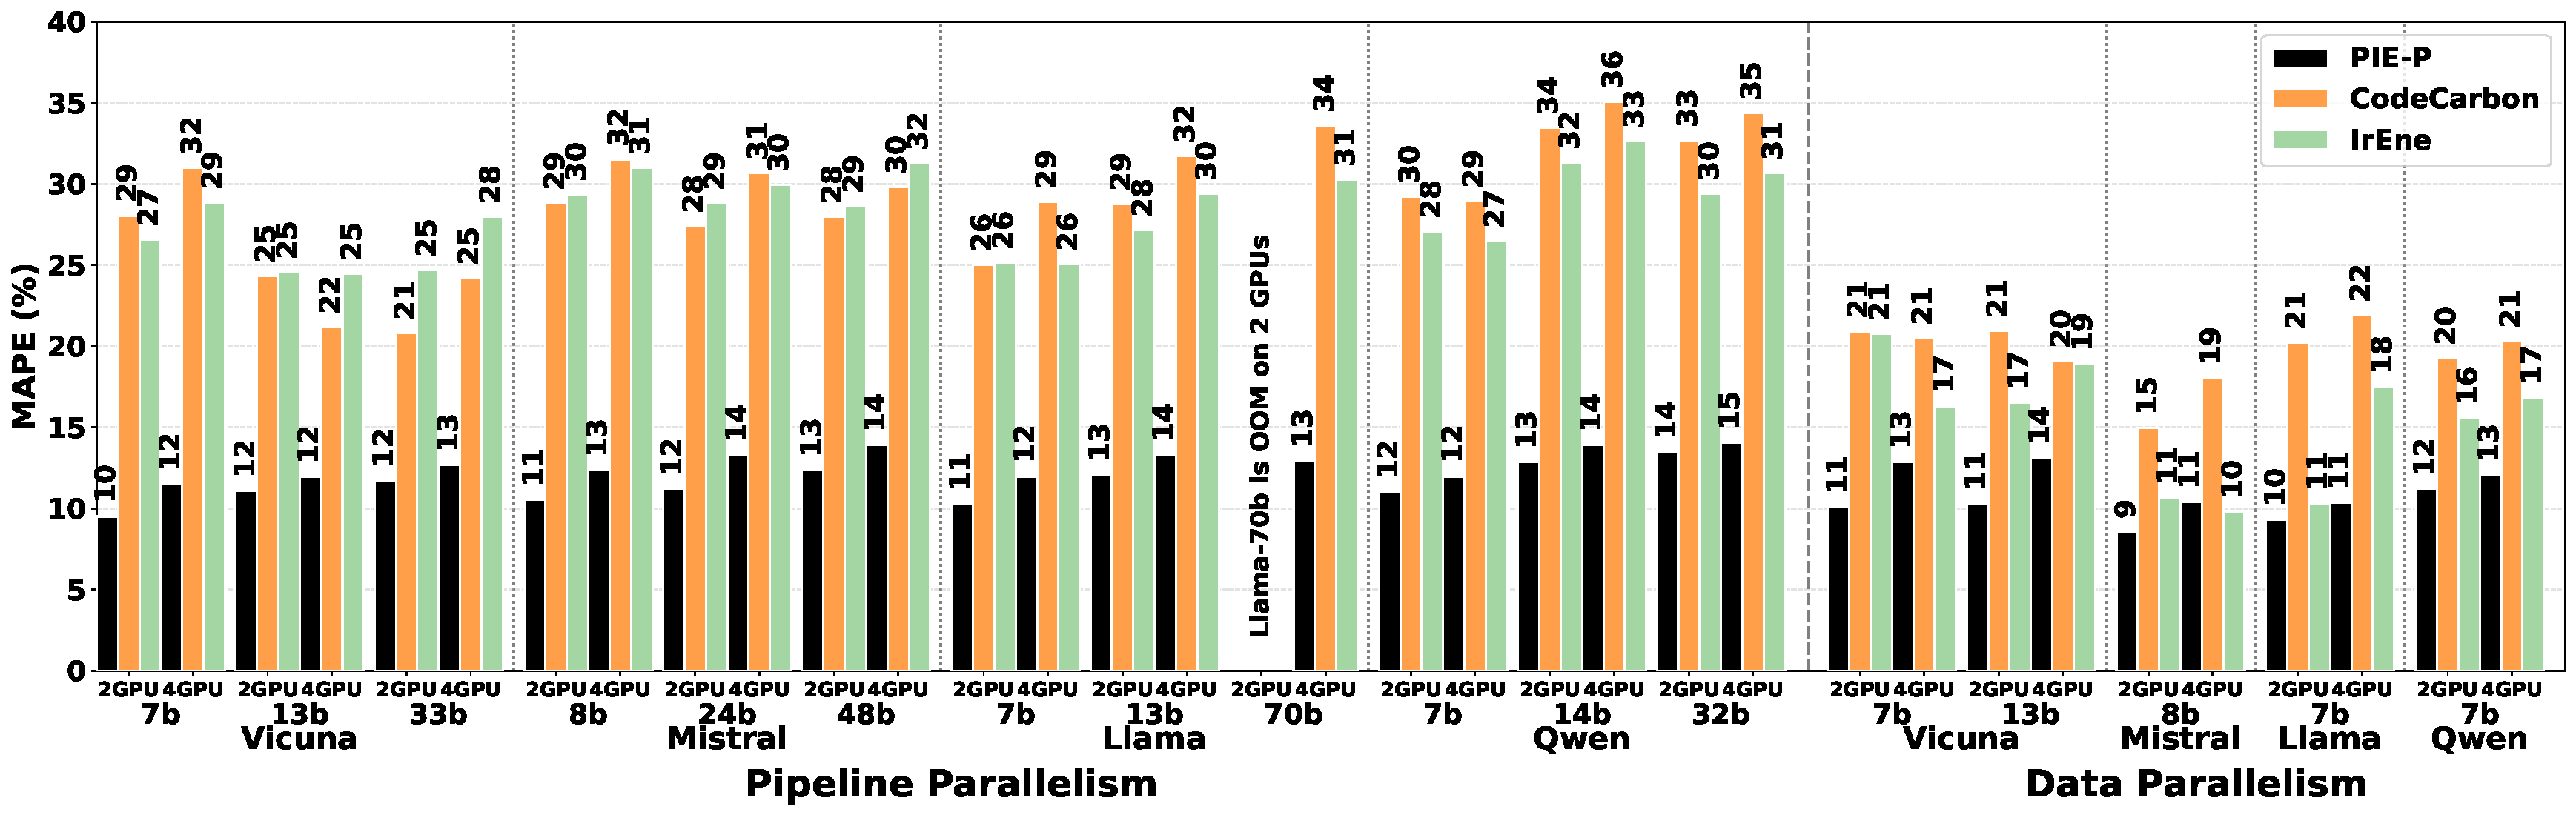
\includegraphics[height=0.22\textwidth,width=0.9\textwidth]{figures/pp_dp_comparison.pdf}
    \vspace{-10pt}
    \caption{MAPE results for all 4 model families under pipeline and data parallelism. Models with the largest parameter sizes in all 4 model families could not be compared for DP as they did not fit in GPU memory.}
    \label{fig:mape_comparison_other}
    \vspace{-18pt}
\end{figure*}

Figure~\ref{fig:mape_comparison_other} compares \sys{} against CodeCarbon and IrEne across all four model families and both 2-GPU and 4-GPU deployments under pipeline and data parallelism. We omit the Wilkins et al.\ baseline as it is consistently inferior to the other baselines (see Figure~\ref{fig:mape_comparison}). We also exclude configurations that do not fit in GPU memory (e.g., Llama-70B on 2 GPUs under pipeline parallelism, and several larger models under data parallelism).

Across all evaluated configurations, \be{\sys{} achieves the lowest prediction error for both parallelism strategies}.
Averaged over all points in Figure~\ref{fig:mape_comparison_other}, \sys{} attains MAPE of 12.2\% under pipeline parallelism and 10.8\% under data parallelism.
The baselines incur higher error: CodeCarbon and IrEne achieve 29.0\% and 28.3\% MAPE under pipeline parallelism, respectively, and 19.6\% and 15.3\% under data parallelism.



Pipeline parallel inference incurs recurring inter-GPU data transfers at every stage boundary.
As the number of GPUs increases (hence more stages), the \emph{frequency} of communication events also increases, making pipeline inference particularly sensitive to unmodeled communication effects.
As a result CodeCarbon and IrEne exhibit large errors, especially under 4-GPU.
Data parallel inference, on the other hand, incurs less frequent and more structured communication.
Thus, the penalty for omitting communication, as in CodeCarbon and IrEne, is smaller than in pipeline parallelism, though still higher than \sys{}.

\review{We use tensor parallelism for the full suite of module-level, leave-one-out, hardware, and ablation experiments because it is the most communication-intensive prediction setting: individual operators are sharded across GPUs and collective communication appears repeatedly inside Transformer blocks. Pipeline parallelism instead communicates activations at stage boundaries, while our data-parallel inference setup has less frequent and more structured output communication. The pipeline- and data-parallel experiments therefore test whether the same \sys{} formulation extends to these different communication structures, while the deeper generalization analysis is concentrated on the more challenging tensor-parallel setting.}

\subsection{Ablation Study: Communication Model}
\label{sec:ablation_comm_modeling}
The \textsc{AvgComm} comparison described in \S\ref{ss:esetup} retains \sys{}'s model-tree decomposition and compute-module predictors while replacing the explicit communication model with an average-power estimate.

\begin{figure*}[t]
    \centering
    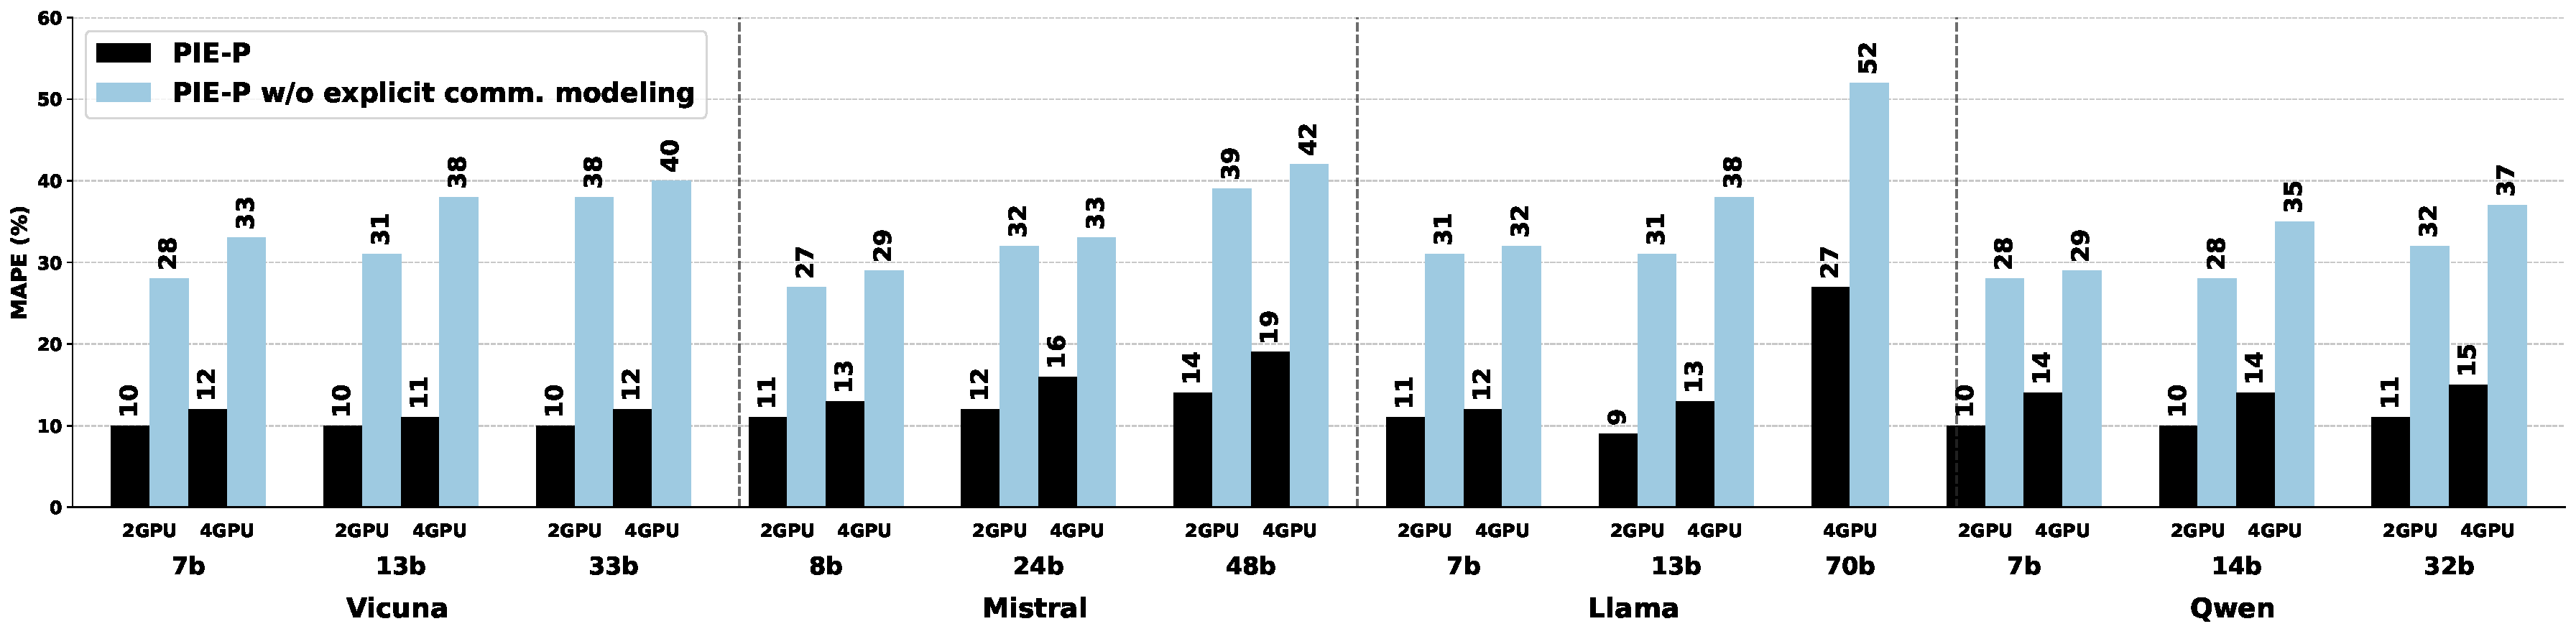
\includegraphics[width=\textwidth]{figures/mape_all_model_families_no_comm_modeling.pdf}
    \vspace{-24pt}
    \caption{Ablation of explicit communication modeling. The ablated variant replaces \sys{}'s communication model with an average communication-power estimate for AllReduce events.}
    \label{fig:ablation_comm_modeling}
    \vspace{-15pt}
\end{figure*}

Figure~\ref{fig:ablation_comm_modeling} shows that \textsc{AvgComm} incurs substantially higher prediction error of 34.0\% compared to \sys{}'s 12.9\%.
The error increase is especially noticeable for larger models and 4-GPU settings, where AllReduce contributes a larger fraction of total energy.
The key distinction is that \sys{} models communication as a first-class module whose features reflect the actual communication.
The \textsc{AvgComm} ablation collapses these differences into a single average value, losing the structure needed to predict communication energy accurately.

\subsection{Ablation Study: Model Tree methodology}
\label{sec:ablation}
We next evaluate the model-level regression comparison described in \S\ref{ss:esetup}, which removes module-level decomposition.

We find that directly predicting total model energy leads to substantially higher errors: the MAPE increases to 61.2\% for Vicuna, 84.3\% for Mistral, 115.1\% for Llama, and 60.8\% for Qwen.
This shows that energy prediction for parallel inference is not simply a model-level regression problem. Runtime features vary significantly across compute-heavy modules (e.g., Attention, MLP) and communication-heavy modules (e.g., AllReduce). Collapsing these effects into a single aggregate feature loses this structure and causes the predictor to mix heterogeneous sources of energy variation.

\anurag{Appendix - K Additional Results: Feature correlation analysis}
\review{\smallskip\noindent\textbf{Feature-correlation analysis.} To assess whether the feature set contributes information beyond one GPU-energy signal, we compute Spearman rank correlations between the candidate features and total measured energy across Vicuna configurations. NVML GPU energy is strongly correlated with total energy ($\rho=0.633$--$0.762$), as expected because GPU computation is a major contributor. However, several non-NVML features are similarly informative: batch size has $\rho=0.735$--$0.737$, execution time has $\rho=0.658$--$0.664$, and memory usage has $\rho=0.656$--$0.663$. Thus, workload size, execution duration, memory activity, and GPU energy all contribute signal; in multi-GPU execution, communication volume and synchronization further perturb these relationships. This supports the multi-feature design rather than a single utilization or telemetry scalar.}

\anurag{Appendix - L Additional Results: Using Latency Prediction Approaches to Predict Energy}
\review{\smallskip\noindent\textbf{Can a latency predictor be retargeted to energy?} Using the NeuSight-style energy predictor described with the baselines above, Table~\ref{tab:neusight_energy_target} shows an average MAPE of 87.3\%, roughly 3--5$\times$ worse than \sys{}. Latency-oriented features describe how long kernels execute but do not explicitly capture power dynamics, system-level energy, inter-GPU communication, or synchronization/waiting effects.}

\begin{table}[t]
\centering
\small
\setlength{\tabcolsep}{6pt}
\renewcommand{\arraystretch}{1.05}
\begin{tabular}{lc}
\toprule
\textbf{Model} & \textbf{MAPE} \\
\midrule
\rowcolor{rowblue} Vicuna 7B  & 79.19\% \\
Vicuna 13B                    & 93.24\% \\
\rowcolor{rowblue} Vicuna 33B & 89.38\% \\
\bottomrule
\end{tabular}
\caption{MAPE for a NeuSight-style latency prediction framework when energy is used as the prediction target.}
\label{tab:neusight_energy_target}
\end{table}

\begin{figure}[t]
    \centering
    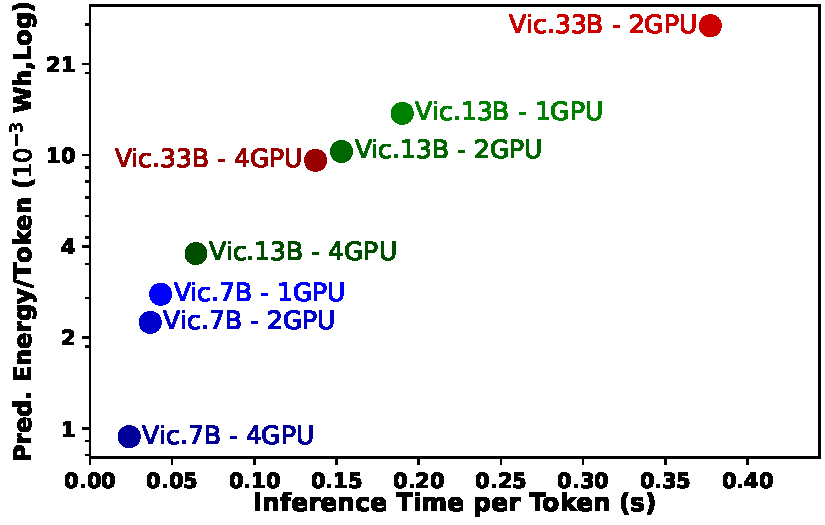
\includegraphics[width=0.40\textwidth]{figures/pareto_plot.pdf}
    \vspace{-9pt}
    \caption{Predicted trade-off between inference time per token and energy per token (log scale) for Vicuna under tensor parallelism.}
    \label{fig:pareto_plot}
    \vspace{-18pt}
\end{figure}
\subsection{Use case: Inference time vs.\ energy for different levels of tensor parallelization}
\label{sec:usecase}

We now present a use case to highlight the applicability of \sys{} in practice.
Consider a setting where an LLM user needs to choose a model and the number of GPUs across which to deploy.
A developer may want to both maximize throughput (i.e., have less time spent on inference per token) and reduce energy consumption.
We show how the user can employ \sys{} to make the right decision.
Figure~\ref{fig:pareto_plot}
illustrates the trade-off between (predicted) energy as a function of inference time for Vicuna models of sizes 7B, 13B, and 33B, across different tensor parallelism configurations (1, 2, and 4 GPUs). We use the highest batch size achievable for each model size. Results are normalized per token and presented on log scale. When compared to ground truth, our prediction errors are around 15\%.

Both per-token energy and inference time increase with model size (7B to 33B), but decrease as the degree of parallelization increases across all three model sizes.
For smaller models such as Vicuna-7B, increasing GPU count from 2 to 4 reduced energy consumption by 43\%, but improved inference time by only 20\%, highlighting diminishing returns. In contrast, larger models like Vicuna-33B benefited more significantly, with a 33\% reduction in energy and a 50\% improvement in speed.
We also extended this analysis to the Qwen family of models, where we found a different scaling efficiency: Qwen-32B achieved 40\% energy reduction when scaling from 2 to 4 GPUs, compared to 33\% for Vicuna-33B, while maintaining similar speedups.

In effect, the energy impact of parallelization is not obvious. Without accurate predictions, model developers require numerous trial-and-error experiments to make energy-conscious parallelization decisions. \sys{} mitigates this effort, providing scalable energy predictions to guide decisions.


\section{Conclusion}
\label{s:conclusion}
Accurate energy prediction enables developers to make energy-aware decisions when selecting LLMs and deployment configurations. To this end, we present \sys{}, a prediction framework that addresses a key gap in accurately predicting the energy of LLMs during parallelized inference. By decomposing the model into its compute and communication modules, designing an accurate inter-GPU communication model, and formulating the prediction problem using a multi-level regressor, PIE-P significantly reduces prediction error across models, hardware platforms, and  three  popular parallelization strategies.
%and demonstrate the utility of the prediction framework for a Pareto-style trade-off analyses for energy-efficient model selection using predicted energies.   

% We acknowledge that \sys{} is hardware-dependent, and one of our immediate next steps is to bridge this hardware dependency gap.
% %so that \sys{} becomes hardware-agnostic, further increasing its practical applicability across diverse deployment scenarios. 
% Through our experiments, we have found hardware-agnostic energy prediction for LLMs to be a challenging task, warranting a full project in itself.
% \sys{} currently supports only decoder-style transformer models. 
% Extending it to encoder-based or encoder-decoder models is left for future work. This is challenging because encoder and encoder-decoder models often have bidirectional attention patterns and different execution flows, which affect both the structure of the model tree and the communication patterns. %Similarly, pipeline and data parallelism introduce distinct synchronization and scheduling behaviors that require new abstractions and measurement strategies.

\section{Future Work}
\label{s:future-work}
% Previous Limitations section retained for reference.
% Our experimental results show that \sys{} generalizes across models and can accurately predict the energy consumption of parallelized inference on different hardware. One limitation in terms of the hardware is that we need to train \sys{} for each hardware as GPU capabilities and architecture can differ significantly. We note that, on the other hand, we do {\em not} have to train a new \sys{} predictor for each model. Our immediate next steps is to bridge this gap so that \sys{} becomes hardware-agnostic, further increasing its practical applicability across diverse deployment scenarios. Through our experiments, we have found hardware-agnostic energy prediction for LLMs to be a challenging task, warranting a full project in itself.
% \sys{} currently supports only decoder-style transformer models. %Extending it to encoder-based or encoder-decoder models is left for future work. 
% Encoder and encoder-decoder models often have bidirectional attention patterns and different execution flows, which affect both the structure of the model tree and the communication patterns. We believe that our parallelization-aware decomposition and communication modeling can be extended to encoder and encoder-decoder models; but we leave this extension for future work. Finally, in this work we show the effectiveness of \sys{} prediction under three popular parallelization strategies. Our next research steps will include extending the prediction to combinations of parallelism strategies such as 3D parallelism as well as other strategies including expert parallelism.
% 
% 
% \begin{comment}
% \begin{itemize}
%     \item only one type of model: vicuna
%     \item only focused on tensor parallelism, not pipeline parallel
%     \item parallel, not distributed
%     \item requires many experiments to collect significant sample size for wait times
%     \item can we call out some further opportunities to improve MAPE, especially for AllReduce?
% \end{itemize}
% \end{comment}

% \review{A next step is to reduce the cost of adapting \sys{} to new GPU platforms. The model-tree decomposition and structural features are reused across A6000, B40, and H200, while communication latency, power, and module-level energy predictors are calibrated for each platform. We will investigate whether limited target-platform profiling can support adaptation without retraining the predictors from scratch.}

\review{Our experimental results show that \sys{} generalizes across model families and accurately predicts the energy of parallelized inference on the evaluated GPU platforms.
%However, \sys{} is trained separately for each hardware as GPU capabilities and architecture can differ significantly.
While the model-tree decomposition and structural features are reused across A6000, B40, and H200, communication latency, power, and module-level energy predictors are calibrated separately for each platform.
A natural next step is to investigate whether limited target-platform profiling can support adaptation without retraining the predictors from scratch.}

% \review{We also plan to extend the model-tree abstraction to additional architectures and parallelism configurations. Encoder-decoder and mixture-of-experts models introduce different module structures and communication operations, while hybrid tensor, pipeline, and data parallelism combines multiple communication patterns. These settings call for corresponding extensions to module decomposition and communication-event calibration.}

\review{We also plan to extend the \sys{} methodology to additional architectures and parallelism configurations.
Encoder-decoder and mixture-of-experts models introduce different module structures and communication operations, while hybrid configurations combining tensor, pipeline, and data parallelism introduce multiple communication patterns.
Predicting energy in these settings will require extending the model-tree decomposition and characterizing the associated computation, communication, and synchronization costs.}

\review{\noindent\textbf{FSDP-style parameter sharding.} Fully Sharded Data Parallel (FSDP), originally developed for training, distributes parameter shards across ranks and all-gathers a module's weights before its forward computation~\cite{zhao2023fsdp}. Extending \sys{} to parameter-sharded inference requires modeling the volume and frequency of weight transfers under different sharding, prefetching, and parameter-retention policies. These transfers can overlap computation, and their energy cost must be distinguished from gradient synchronization, which is specific to training.}

\review{\noindent\textbf{Context parallelism.} Context-parallel methods distribute long sequences across GPUs, using schemes such as ring exchanges of attention key/value blocks~\cite{liu2023ringattention} or all-to-all redistribution of attention tensors~\cite{jacobs2023deepspeedulysses}. Predicting inference energy under these strategies requires modeling context-length-dependent attention work, per-GPU key/value storage, and communication schedules. Their potential overlap between attention computation and data transfers introduces additional energy-attribution challenges.}


% =========================================================
% References
% =========================================================
\bibliographystyle{IEEEtran}
\bibliography{custom}

% =========================================================
% Appendix (disabled for IPDPS submission)
% =========================================================
% \appendix
% % \section{Background: AllReduce, AllGather, and Point-to-Point communication}
% \label{app:collective-background}

% In this section, we provide details of the communication patterns used in tensor, pipeline and data parallelism strategies. 
% %\sys{} extends the model tree abstraction of IrEne by introducing a dedicated module for AllReduce operations, which is essential for capturing the energy dynamics of tensor-parallelized inference. This extension is necessary because AllReduce operations introduce unique energy consumption patterns tied to inter-GPU communication that cannot be captured by the existing math, ML, or module level nodes.

% \subsection{AllReduce in tensor parallelism}
% \label{app:tp-ar}

% Tensor parallelism uses a ring-based communication pattern. In the ring AllReduce algorithm, GPUs are arranged in a logical ring structure where each GPU communicates only with its immediate neighbors, reducing global communication overhead. The operation proceeds in two distinct phases:

% \begin{enumerate}
%     \item \textbf{ReduceScatter Phase}: Each GPU divides its data into equal chunks (one per GPU). In this phase, each GPU sends a chunk to its successor in the ring and receives a chunk from its predecessor. Upon receiving data, each GPU performs a reduction operation (e.g., sum) with its corresponding local chunk. This process continues for $n-1$ steps (where $n$ is the number of GPUs), at which point each GPU has one fully reduced chunk of the final result.
    
%     \item \textbf{AllGather Phase}: In this phase, the reduced chunks are disseminated to all GPUs. Each GPU sends its reduced chunk to its successor and receives a different reduced chunk from its predecessor. After $n-1$ steps, all GPUs have all chunks of the fully reduced data.
% \end{enumerate}

%There are two phases of the AllReduce process that is captured by the model abstraction tree:
%
%\begin{enumerate}
%    \item \textbf{Communication Nodes}: Capturing the data transfers between adjacent GPUs in the ring.
%    \item \textbf{Synchronization Nodes}: Modeling the waiting periods where faster GPUs idle while waiting for slower ones to complete their operations.
%\end{enumerate}

% \subsection{Point-to-Point Data Transfers in Pipeline Parallelism}
% \label{app:pp-p2p}

% In pipeline parallelism, stage $i$ sends its forward activations to stage $i{+}1$ via \emph{point-to-point} device-to-device transfers (e.g., NVLink/PCIe/Ethernet). 
% During inference there are no gradients; the only communication are the hop-local activation sends/receives. 
% Operationally, the transfer for a given microbatch occurs immediately after stage $i$ finishes its forward compute and before stage $i{+}1$ launches its first kernel on the received activations. 
%We profile this communication by timestamping (with \texttt{nsys}) the end of stage~$i$’s last forward kernel and the start of stage~$i{+}1$’s first forward kernel; the interval between these two events is attributed to the Point-to-Point transfer. 
%We integrate power over this window to obtain P2P energy, repeating across hops and microbatches to form robust aggregates. Because these are explicit, hop-local sends/recvs rather than collectives, timing variability is typically small, and the attribution is more deterministic than in tensor-parallel synchronization phases.


% \subsection{All Gather in data parellelism}
% \label{app:dp-allgather}

% In data parallelism, each replica computes the full forward pass for its local microbatch and then \emph{collates the final outputs} (e.g., logits/token scores) across replicas with a single AllGather at the end of inference. Mechanistically, the last layer on each GPU (typically the output projection / logits head) finishes, the runtime immediately exchanges each replica’s output tensor, and the concatenated result is handed to the host for post-processing (sampling, metrics, or write-out). 
%This makes profiling straightforward: \emph{profiling the output layer automatically profiles the AllGather}, since it is the next and final step. 
%This collation is a \emph{single, tail-end} exchange of \emph{final outputs} (logits/token scores) whose tensors are much smaller than hidden activations, and it happens once per request (or per decode step). 
    % By contrast, Pipeline P ships \emph{activations between every adjacent stage} for each microbatch, and TP executes \emph{layer-internal collectives} (e.g., reduce–scatter/all-gather) on large hidden states multiple times per layer—hence substantially higher communication volume and energy in PP/TP than in DP.


\section{Methodology: Data Collection to predict communication energy}
\label{app:data-collection-parallel}
We describe the methodology we use to collect data to build a communication energy prediction model. Since communication is different for different parallelism strategies, we describe our data collection method for each parellism strategy below.

\paragraph{Tensor Parallelism (TP)}: During profiling, we capture the \emph{full distribution} of energy consumption caused by non-deterministic GPU synchronization through multiple runs. 
  By capturing a distribution of GPU wait times, rather than relying on a single execution run, we ensure that \sys{} reflects both leading and lagging GPU behavior, \be{accounting for variability}.
  We specifically capture the distribution of 
  %NCCL's (Nvidia Collective Communication Library) ring 
  the ring \textbf{AllReduce} operation, which consists of (i) ReduceScatter: GPUs exchange neighbor chunks and reduce for $n{-}1$ steps until each holds one fully-reduced shard, followed by (ii) AllGather: GPUs circulate these shards for $n{-}1$ steps so all ranks recover the full tensor. 
  The abstraction includes both \emph{communication} (hop transfers) and \emph{synchronization} (idle/wait due to stragglers), since AllReduce energy is shaped by link activity and barrier-induced stalls.

\paragraph{Pipeline Parallelism (PP)}: We capture data transfer by benchmarking the interval between completion of boundary layer in the producing stage and start of the next stage in the next GPU. 
    The only inference-time communication is \textbf{point-to-point} (P2P) activation transfers from stage $i$ to $i{+}1$ after stage $i$ finishes its forward kernels and before stage $i{+}1$ starts compute on received activations. 
    We profile each hop by timestamping (via \texttt{nsys}) the end of stage $i$’s last forward kernel and the start of stage $i{+}1$’s first forward kernel; the intervening interval is attributed to P2P transfer, and power is integrated over this window to estimate P2P energy.

\paragraph{Data Parallelism} Since each replica produces its own output, profiling the final output stage (\textbf{AllGather}) is sufficient to capture communication energy. Replicas run full forward passes independently and perform a single tail-end AllGather operation to collate final outputs (e.g., logits/token scores) across GPUs; this exchange occurs immediately after the output layer completes, making attribution straightforward and typically lower-volume than TP/PP communication.

\section{Methodology: Features}
\label{appendix:features}

\begin{table}[t]
\centering
\small
\setlength{\tabcolsep}{4pt}
\renewcommand{\arraystretch}{1.05}

\begin{tabular}{@{}
>{\raggedright\arraybackslash}p{0.48\linewidth}
>{\raggedright\arraybackslash}p{0.48\linewidth}
@{}}
\toprule
\rowcolor{rowblue}
\multicolumn{2}{@{}l@{}}{\textbf{Resource Utilization Features}}\\
\midrule
CPU utilization (\%) & CPU mem. utilization (\%)\\
\rowcolor{rowblue} GPU utilization (\%) & GPU mem. utilization (\%)\\
CPU clock (GHz) & CPU mem. clock (GHz)\\
\rowcolor{rowblue} Memory (bytes) & GPU clock (GHz)\\
GPU mem. clock (GHz) & \\
\midrule

\rowcolor{rowblue}
\multicolumn{2}{@{}l@{}}{\textbf{Execution Features}}\\
\midrule
Batch size & Sequence length\\
\rowcolor{rowblue} FLOPs per token (billions) & Execution time (s)\\
GPU energy NVML (Wh) & Number of GPUs\\
\midrule

\rowcolor{rowblue}
\multicolumn{2}{@{}l@{}}{\textbf{Model Structure Features}}\\
\midrule
Feed-forward dimension & Transformer blocks\\
\rowcolor{rowblue} Hidden embedding size & Attention heads\\
Key-value heads & \\
\midrule

\rowcolor{rowblue}
\multicolumn{2}{@{}l@{}}{\textbf{Communication Features}}\\
\midrule
Bytes transferred & Effective bandwidth \\
% \rowcolor{rowblue} Hidden embedding size & Attention heads\\

\bottomrule
\end{tabular}
\vspace{-9pt}
\caption{Features used by \sys{} for prediction.}
\label{tab:features}
\vspace{-17pt}
\end{table}

Table~\ref{tab:features} summarizes these features, grouped into resource utilization (captures system- and device-level activity during inference), execution parameters (capture the workload configuration that drives runtime/energy), and model structure (captures architectural properties that determine tensor sizes). 
For communication modules, we additionally collect communication-specific features: the bytes sent, the bytes received, and the effective bandwidth for each inter-GPU communication event.

% \section{Methodology Alpha--Beta Model for Communication Energy}
% \label{app:alpha-beta-comm}
% \aruna{can potentially be removed, content is moved to main text}
% {
% PIE-P models collective communication using an offline-calibrated alpha--beta latency predictor. For a communication event $e$ of operation type $o$ running on $p$ GPUs, let $B_{e}^{\mathrm{out}}$ and $B_{e}^{\mathrm{in}}$ denote the bytes sent and received by each rank. The total per-rank communication volume is:
% }
% \begin{equation}
% \label{eq:comm-volume}
% V_e =
% B_{e}^{\mathrm{out}} + B_{e}^{\mathrm{in}} .
% \end{equation}
% The communication latency is then predicted as
% \begin{equation}
% \label{eq:alpha-beta-comm}
% T*{e}^{\mathrm{comm}} =
% \alpha*{o,p} + \beta_{o,p} V_e .
% \end{equation}
    % {}
% Here, $\alpha_{o,p}$ captures fixed launch, scheduling, and synchronization overheads, while $\beta_{o,p}=1/B_{o,p}^{\mathrm{eff}}$ captures the inverse effective bandwidth. For ring AllReduce with tensor size $S_e$, each rank sends and receives $(p-1)S_e/p$ bytes. Thus, the AllReduce communication volume is
% \begin{equation}
% \label{eq:allreduce-volume}
% V_e^{\mathrm{AR}} =
% \frac{2(p-1)}{p}S_e .
% \end{equation}
% The AllReduce latency prediction is
% \begin{equation}
% \label{eq:allreduce-latency-short}
% T*{e}^{\mathrm{AR}} =
% \alpha*{\mathrm{AR},p}
% +
% \beta_{\mathrm{AR},p} V_e^{\mathrm{AR}} .
% \end{equation}

% PIE-P converts predicted communication latency into energy using calibrated average communication power. For an AllReduce event, the predicted energy is
% \begin{equation}
% \label{eq:allreduce-energy-short}
% E*{e}^{\mathrm{AR}} =
% \frac{P*{\mathrm{AR},p}^{\mathrm{comm}}
% T*{e}^{\mathrm{AR}}}{3600}.
% \end{equation}
% The total compute and communication energies are
% \begin{equation}
% \label{eq:total-compute-energy-short}
% E^{\mathrm{compute}} =
% \sum*{m \in \mathcal{M}}
% E*{m}^{\mathrm{compute}} .
% \end{equation}
% \begin{equation}
% \label{eq:total-comm-energy-short}
% E^{\mathrm{comm}} =
% \sum*{e \in \mathcal{C}}
% E*{e}^{\mathrm{comm}} .
% \end{equation}
% The final model-level prediction is
% \begin{equation}
% \label{eq:model-energy-alpha-beta-short}
% E*{\mathrm{model}} =
% R\left(
% E^{\mathrm{compute}} +
% E^{\mathrm{comm}}
% \right).
% \end{equation}
% This formulation captures both the fixed overhead and message-size-dependent cost of inter-GPU communication without requiring online communication-energy sampling during inference.

\section{Methodology: Details of predicting communication energy}
\label{app:alpha-beta-comm}

Section~\ref{ss:design-communication} introduces the $\alpha$-$\beta$ communication model used by \sys{} in Eq.~\ref{eq:comm-latency-main}. 
Here, we provide the details for computing the communication-volume term $\left(B_{e}^{\mathrm{out}} + B_{e}^{\mathrm{in}}\right)$ and the effective-bandwidth parameter $\beta_{o,p}$ used in that equation.

For a communication event $e$ of operation type $o$ running on $p$ GPUs, let $B_{e}^{\mathrm{out}}$ and $B_{e}^{\mathrm{in}}$ denote the bytes sent and received by each GPU. 
The total per-GPU communication volume is:
\vspace{-9pt}
\begin{equation}
\label{eq:comm-volume}
V_e =
B_{e}^{\mathrm{out}} + B_{e}^{\mathrm{in}} .
\vspace{-9pt}
\end{equation}

We calibrate the effective bandwidth offline for each communication operation $o$ and GPU count $p$. 
For each calibration run, we record the communication volume $V_e$ and the observed communication time $T_{e}^{\mathrm{obs}}$. 
We then fit the alpha-beta relation:
\vspace{-9pt}
\begin{equation}
\label{eq:alpha-beta-calibration}
T_{e}^{\mathrm{obs}} =
\alpha_{o,p} +
\beta_{o,p} V_e .
\vspace{-9pt}
\end{equation}
Here, $\alpha_{o,p}$ captures fixed communication overheads, while $\beta_{o,p}$ captures the message-size-dependent transfer cost. 
The corresponding effective bandwidth is:
\vspace{-9pt}
\begin{equation}
\label{eq:effective-bandwidth}
B_{o,p}^{\mathrm{eff}} =
\frac{1}{\beta_{o,p}} .
\vspace{-9pt}
\end{equation}

For ring AllReduce, if the communicated tensor has size $S_e$ bytes, each GPU sends and receives $(p-1)S_e/p$ bytes across the ReduceScatter and AllGather phases. 
Thus, the total per-GPU AllReduce communication volume is:
\vspace{-9pt}
\begin{equation}
\label{eq:allreduce-volume}
V_e^{\mathrm{AR}} =
\frac{2(p-1)}{p}S_e .
\vspace{-9pt}
\end{equation}
This volume is used as the communication-volume input for AllReduce events in Eq.~\ref{eq:comm-latency-main}. 
For pipeline-parallel point-to-point transfers and data-parallel AllGather operations, we apply the same accounting procedure using the tensor size and the corresponding communication pattern described in Appendix~\ref{app:collective-background}.


\section{Methodology: Training }
\label{app:training_methodology}

Our detailed training methodology is described below. We use a hierarchical approach, first training module-level predictors and then combining them for model-level prediction. We employed 3-fold cross-validation at the module level, training on 70\% of datapoints while testing on the remaining 30\%. 

Each module (e.g., Self-Attention, MLP, AllReduce) is sampled $10{,}000$ times to build a robust dataset. A single sample corresponds to one aggregated measurement obtained by running the module $100{,}000$ times in a specific GPU configuration setting. For each sampling run, we compute the mean, standard deviation, minimum, and maximum values of these features across all participating GPUs to account for runtime variance and workload imbalance. These are combined with structural features to form the complete feature vector for each sample.

To ensure that the models are evaluated under varied operational conditions, we perform sampling across multiple output configurations. Specifically, for each model variant, we run experiments using batch sizes of 8, 16, 32, and 64, and output sequence lengths of 512 and 1024. This sampling regime captures both low and high throughput scenarios, improving the robustness and generalizability of our predictors. We use Deepspeed \citep{deepspeed}, a widely used inference serving python library to run our tests for all parallelism modalities.


For each model family (e.g., Vicuna), we combined module-level energy predictions across all variants using the extracted features. The model-level energy prediction was composed using the regression formula: 
% $\text{model\_energy} = \text{regression}(\text{self\_attention\_energy} + \text{MLP\_energy} + \text{AllReduce\_energy} + \ldots)$.


\vspace{-9pt}
\setlength{\abovedisplayskip}{2pt}
\setlength{\belowdisplayskip}{2pt}
\begin{equation}
\begin{aligned}
E_{\text{model}} = \mathcal{R}(&E_{\text{attn}} + E_{\text{MLP}} \\
&+ E_{\text{AllReduce}} + \ldots)
\end{aligned}
\vspace{-6pt}
\end{equation}
% \vspace{-9pt}

%For the \sys{} without waiting phase baseline, we substituted the AllReduce module's predicted energy with just the network transfer predicted energy, excluding the waiting phase component. For the IrEne baseline, we excluded AllReduce energy completely from the regression. 
%\label{app:use-case-ground-truth}

%Figure~\ref{fig:mape_comparison} reports the MAPE values obtained from this regression, where each model-level energy prediction MAPE is derived from a regression over its module-level energy components. The error bars represent the standard errors computed over the individual percentage errors of each prediction.



%\label{app:module_mape}
%For each model variant, we obtain module-level energy MAPE values (in Table ~\ref{tab:module_mape_comparison} by running each module type (e.g., Self-Attention, MLP, AllReduce) multiple times under varying input configurations and computing their predicted energy values. If a module appears multiple times in a model (e.g., multiple Feed Forward Networks), we first average the predicted energies across those instances. The final MAPE for a module type is then averaged across all variants and across all four model families.

%\begin{figure}[t]
 %   \centering
  %  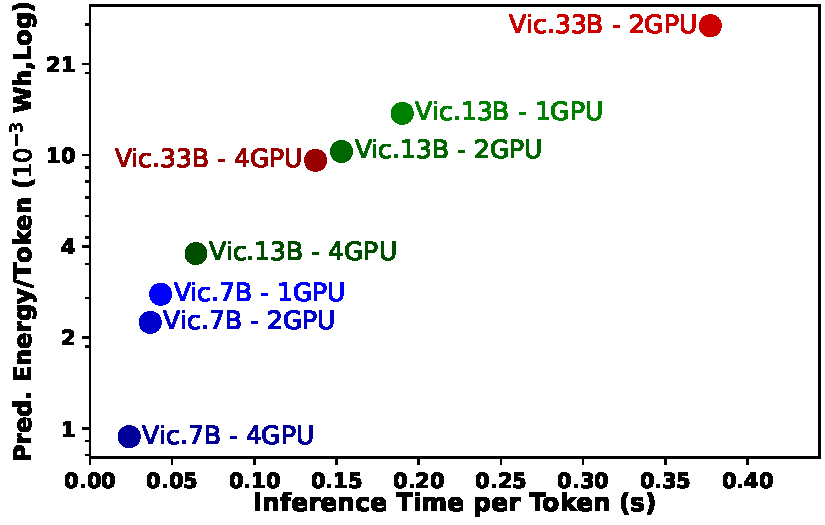
\includegraphics[width=\columnwidth]{figures/pareto_plot.pdf}
  %  \caption{Ground truth energy trade-off between inference time per token and energy per token (on log scale) for Vicuna under tensor parallelism.}
  %  \label{fig:pareto_plot_ground_truth}
%\end{figure}
%Figure~\ref{fig:pareto_plot_ground_truth} shows the trade-off between actual energy consumption and inference time per token across Vicuna model sizes and GPU configurations.
%\label{app:generalization-unseen-variants}

To evaluate generalization across unseen model variants (Appendix~\ref{app:additional-generalization-unseen-variants}), we adopt a leave-one-variant-out strategy. Specifically, for each experiment, we exclude one model variant entirely from training and train a model-level energy regressor using the predicted module-level energies from the remaining variants within the same model family. During evaluation, we predict the total energy of the held-out variant using its module-level energy predictions as input. This setup allows us to assess the ability of \sys{} to generalize across model scales and configurations within a family.




\section{Evaluation: Baselines}
\label{app:baselines}

In this section, we describe the baselines we use to compare with \sys{} in more detail. 

\textbf{IrEne}~\citep{irene} is a multi-level energy prediction model that combines fine-grained model execution features with resource utilization for more accurate energy prediction.  
IrEne first constructs a model tree abstraction that captures the model's computational structure at three levels: math level, machine learning (ML) level, and module level. 
The math level consists of basic mathematical operations like matrix multiplication and addition, which are model-agnostic and can generalize across various models. 
The operations at the ML level nodes, such as Linear and LayerNorm, are more specific to ML tasks but are still generalizable. 
The module level nodes (e.g., SelfAttention) are higher-level nodes that are made up of several ML tasks combined together. 

 
IrEne then uses a bottom-up prediction approach for energy estimation. At the leaf level, IrEne learns the energy consumption of each node using features derived from runtime resource utilization (e.g., GPU usage) and model specifications (e.g., input size). IrEne uses ground truth measurement for training. At each intermediate node going up to the root, energy predictions are recursively computed by combining the predicted energy values of child nodes through a single regressor.

\textbf{CodeCarbon}: Software based energy estimator that tracks runs via readily available telemetry (e.g., GPU via NVML, CPU via RAPL/powermetrics) and integrates power over time to report kWh (and optionally emissions). CodeCarbon is currently state-of-the-art for software-based energy estimation and is used by researchers and practitioners for system-level energy/emissions estimation~\cite{Jesse-dodge-icml}.

\textbf{Wilkins et. al}: Energy estimator that learns coefficients based on token-in/token-out energy ratios. We implement this token-in/token-out regression technique, illustrated in  
%which predicts per-request energy as a function of input and output token counts with an interaction term in 
Eq.~(\ref{eq:wilkins-tok2e}), where the coefficients $(\alpha_0,\alpha_1,\alpha_2)$ are fit from a calibration set. This is included as a recent, deployment-friendly baseline that estimates energy without hardware monitors. 
% \begin{wrapfigure}[3]{r}{0.48\linewidth}
% 
% \begin{minipage}{\linewidth}
% \setlength{\abovedisplayskip}{4pt}\setlength{\belowdisplayskip}{4pt}
\vspace{-6pt}
\setlength{\abovedisplayskip}{2pt}
\setlength{\belowdisplayskip}{2pt}
\begin{equation}
\begin{aligned}
e_K(\tau_{\mathrm{in}}, \tau_{\mathrm{out}})=\;&\alpha_0\,\tau_{\mathrm{in}}+\alpha_1\,\tau_{\mathrm{out}}
+\alpha_2\,\tau_{\mathrm{in}}\tau_{\mathrm{out}}
\end{aligned}
\label{eq:wilkins-tok2e}
\vspace{-6pt}
\end{equation}
% \vspace{-9pt}

\textbf{NVML}: NVML is a software based GPU status tracking software that allows for real time metrics such as temperature, power, and memory utilization. We implement a linear regressor at the model level using NVML-collected energy as the independent variable and total energy consumed as the dependent variable. 



%\section{Additional results: AllReduce energy consumption }
%\label{app:allreduce-energy}
%
%\begin{figure*}[t]
%\centering
%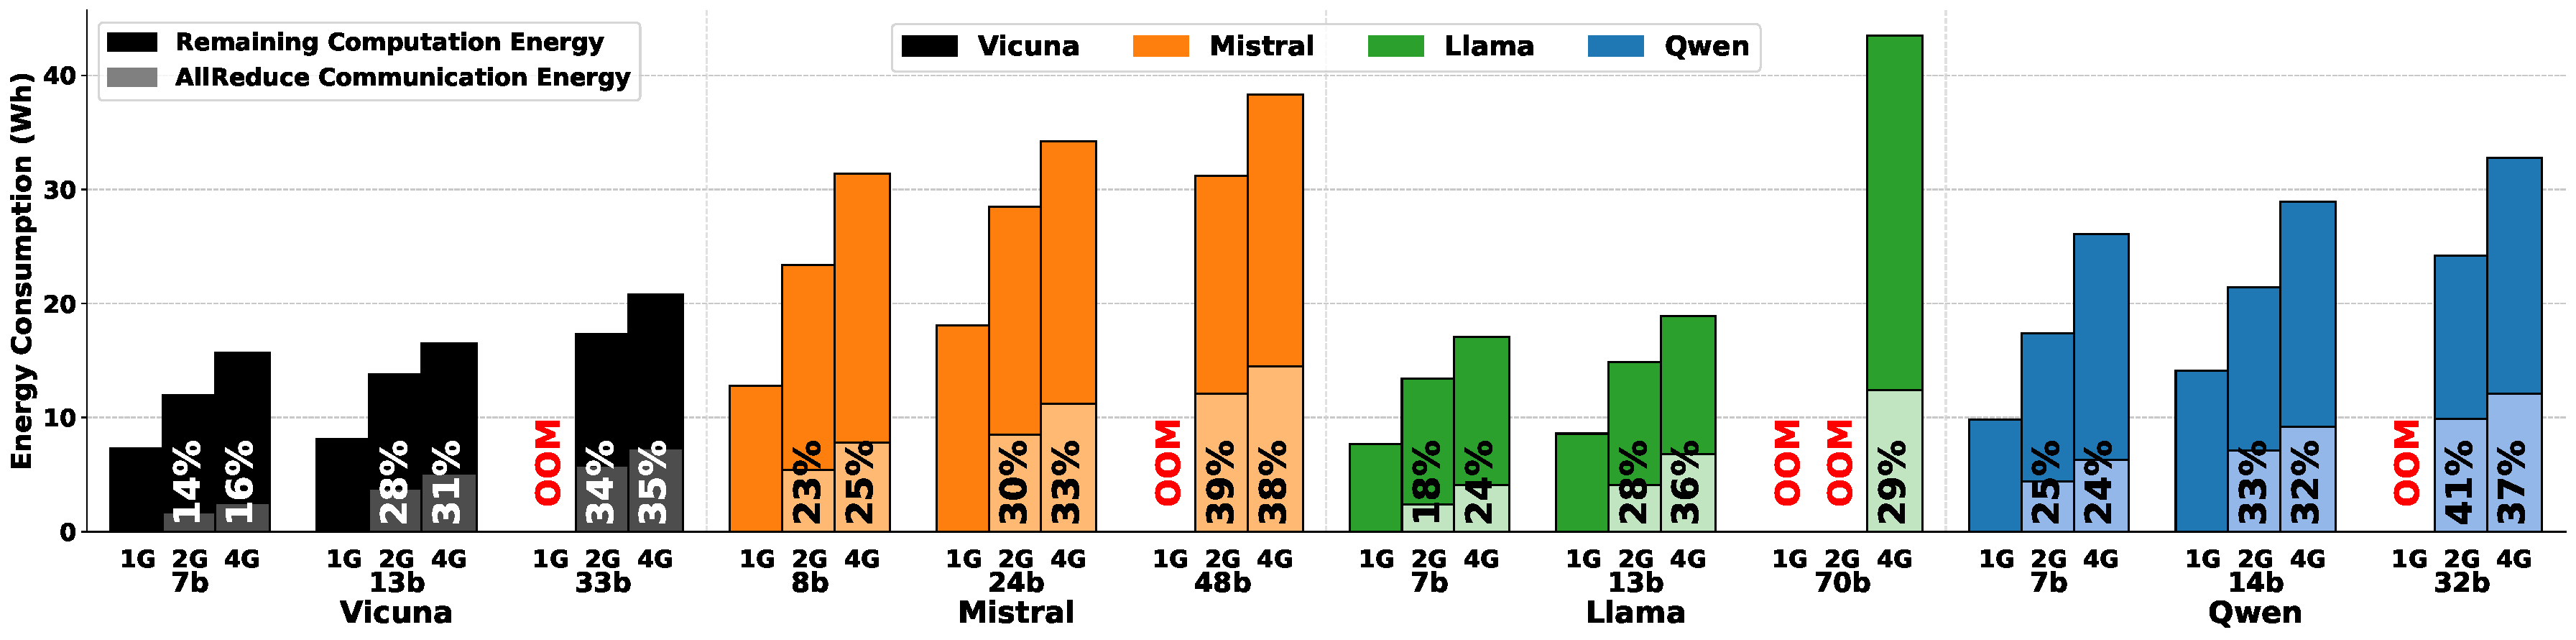
\includegraphics[width=\textwidth]{figures/llm_energy_comparison.pdf}
%\caption{Energy consumption across different model families and GPU configurations. The bars show total energy consumption per model with lighter-colored segments representing AllReduce communication energy (\% shown) and darker segments showing remaining computation energy.}
%\label{fig:all_reduce_ratio}
%\vspace{-6pt}
%\end{figure*}
%
%
%Figure~\ref{fig:all_reduce_ratio} shows the energy consumption breakdown for parallelized inference across different GPU configurations for four model families: Vicuna, Mistral, Llama, and Qwen. Across all model families, AllReduce consumes a considerable amount of energy both for 2 to 4 GPUs in tensor-parallel configurations for batched inferences. For example, for the Vicuna family, the AllReduce energy constitutes 14.2\% (1.7 Wh/12.0 Wh) of total energy with 2 GPUs for the 7B model, increasing to 15.9\% (2.5 Wh/15.7 Wh) with 4 GPUs. This proportion is higher for larger models, reaching 27.5\% (5.8 Wh/17.3 Wh) for Vicuna-33B with 2 GPUs and 35.1\% (7.3 Wh/20.8 Wh) with 4 GPUs.
%
%We observe that the proportion of AllReduce energy correlates strongly with the complexity of the transformer architecture. Models with more sophisticated attention mechanisms and larger feed-forward dimensions, such as Mistral and Qwen, show significantly higher AllReduce energy proportions compared to models with simpler architectures like Vicuna. More complex transformer blocks lead to higher AllReduce energy proportions because they generate larger intermediate tensors that must be synchronized across GPUs. 
%For instance, Mistral-8B employs grouped-query attention with 32 attention heads but only 8 key-value heads, resulting in approximately 245 GFLOPs per transformer block—31\% higher than Vicuna-7B's 187 GFLOPs per block with standard self-attention and 32 attention heads. As a result, the proportional energy consumption of AllReduce for Mistral is higher.


% \section{Additional results: NVML generalization for energy prediction}
% \label{app:nvml_generalization}
% \begin{table}[t]
% \centering
% \small
% \setlength{\tabcolsep}{3pt}
% \renewcommand{\arraystretch}{1.05}

% \begin{tabular}{
%   @{}
%   l
%   c
%   l
%   c
%   @{}
% }
% \toprule
% \textbf{Model} & \textbf{MAPE} & \textbf{Model} & \textbf{MAPE} \\
% \midrule
% \rowcolor{rowblue} Vicuna 7B   & 48.3\% & Llama 7B   & 47.4\% \\
% Vicuna 13B                     & 51.1\% & Llama 13B  & 49.1\% \\
% \rowcolor{rowblue} Vicuna 33B  & 50.0\% & Llama 70B  & 53.4\% \\
% \midrule
% Mistral 8B                     & 57.3\% & Qwen 8B    & 51.1\% \\
% \rowcolor{rowblue} Mistral 24B & 52.1\% & Qwen 14B   & 49.2\% \\
% Mistral 48B                    & 51.3\% & Qwen 32B   & 56.5\% \\
% \bottomrule
% \end{tabular}

% \caption{Leave-one-out generalization results for NVML-based regression. Each row shows MAPE when using NVML measurements to predict total energy for a model excluded from training. The high error rates, ranging from 47.4\% to 57.3\%, demonstrate NVML's poor generalization capabilities.}
% \label{tab:nvml_loo}
% \end{table}

% Beyond examining NVML's limitations as a direct proxy for total energy, we also evaluated its generalization capabilities using leave-one-out cross-validation. Table~\ref{tab:nvml_loo} shows the results when NVML-based regression models are trained on all models of the same model family except one, then tested on the excluded model.

% The results reveal significantly higher prediction errors compared to both in-sample NVML prediction (29.8-44.2\% MAPE) and \sys{}'s leave-one-out performance (15.8-24.5\% MAPE). MAPE values range from 47.4\% to 57.3\%, with an average of 51.5\% across all models (Table ~\ref{tab:nvml_loo}). These poor generalization results further reinforce our conclusion that GPU-only measurements are insufficient for accurate energy prediction in tensor-parallelized settings, particularly when generalizing to new model architectures or configurations. The substantial gap between \sys{} and NVML generalization performance (average improvement of 31.5 percentage points) demonstrates the critical importance of our approach's architecture-aware features and synchronization modeling.

\section{Additional results: NVML as a proxy for total energy}
\label{app:nvml_proxy}
\begin{table}[t]
\centering
\small
\setlength{\tabcolsep}{3pt}
\renewcommand{\arraystretch}{1.05}

\begin{tabular}{
  @{}
  l
  c
  l
  c
  @{}
}
\toprule
\textbf{Model} & \textbf{MAPE} & \textbf{Model} & \textbf{MAPE} \\
\midrule
\rowcolor{rowblue} Vicuna 7B   & 33.4\% & Llama 7B   & 31.1\% \\
Vicuna 13B                     & 31.4\% & Llama 13B  & 31.3\% \\
\rowcolor{rowblue} Vicuna 33B  & 29.8\% & Llama 70B  & 28.5\% \\
\midrule
Mistral 8B                     & 44.2\% & Qwen 8B    & 42.4\% \\
\rowcolor{rowblue} Mistral 24B & 40.3\% & Qwen 14B   & 38.0\% \\
Mistral 48B                    & 39.0\% & Qwen 32B   & 38.3\% \\
\bottomrule
\end{tabular}

\caption{MAPE when using NVML-reported GPU energy as a proxy for total system energy. This approach produces substantially higher errors compared to \sys{}. Experiments conducted on A6000s}
\label{tab:nvml_proxy}
\end{table}

Hardware vendors provide built-in power measurement interfaces such as NVIDIA Management Library (NVML) that report GPU-only energy consumption. Can these readily-available measurements be reliable proxies for total system energy through simple regression techniques? % potentially eliminating the need for specialized prediction frameworks. 
%To investigate this approach, we conducted an experiment using NVML-reported GPU energy values as the sole predictor for total system energy consumption.


Table~\ref{tab:nvml_proxy} shows the results when NVML is used to predict total energy. %Despite the apparent simplicity of using NVML measurements directly, 
Prediction errors across all model families and sizes are high. Vicuna models' MAPE range from 29.8\% to 33.4\%, while Mistral's are even higher between 39.0\% and 44.2\%. 
%NVML also generalizes poorly to unseen models, as shown in Appendix~\ref{app:nvml_generalization}.
%The result shows that tensor-parallelized inference energy involves complex interactions between computation, synchronization, and system-level dynamics that cannot be captured by GPU-only measurements alone. % In particular, NVML fails to account for several key factors: (1) CPU energy consumption during scheduling and orchestration, (2) detailed runtime metrics obtained through telemetry and tracing that reveal resource utilization patterns, and (3) model structural features that influence energy consumption across different tensor-parallel configurations. \sys{}'s superior performance demonstrates the necessity of a specialized prediction framework that explicitly models these tensor-parallelism-specific energy dynamics rather than relying on simplified proxy measurements.


%\section{Additional results: NVML generalization for energy prediction}
%\label{app:nvml_generalization}


\begin{table}[t]
\centering
\small
\setlength{\tabcolsep}{3pt}
\renewcommand{\arraystretch}{1.05}

\begin{tabular}{
  @{}
  l
  c
  l
  c
  @{}
}
\toprule
\textbf{Model} & \textbf{MAPE} & \textbf{Model} & \textbf{MAPE} \\
\midrule
\rowcolor{rowblue} Vicuna 7B   & 48.3\% & Llama 7B   & 47.4\% \\
Vicuna 13B                     & 51.1\% & Llama 13B  & 49.1\% \\
\rowcolor{rowblue} Vicuna 33B  & 50.0\% & Llama 70B  & 53.4\% \\
\midrule
Mistral 8B                     & 57.3\% & Qwen 8B    & 51.1\% \\
\rowcolor{rowblue} Mistral 24B & 52.1\% & Qwen 14B   & 49.2\% \\
Mistral 48B                    & 51.3\% & Qwen 32B   & 56.5\% \\
\bottomrule
\end{tabular}

\caption{Leave-one-out generalization results for NVML-based regression. Each row shows MAPE when using NVML measurements to predict total energy for a model excluded from training. The high error rates, ranging from 47.4\% to 57.3\%, demonstrate NVML's poor generalization capabilities. Experiments conducted on A6000s}
\label{tab:nvml_loo}
\end{table}

Beyond examining NVML's limitations as a direct proxy for total energy, we also evaluated its generalization capabilities using leave-one-out cross-validation. Table~\ref{tab:nvml_loo} shows the results when NVML-based regression models are trained on all models of the same model family except one, then tested on the excluded model.

The results reveal significantly higher prediction errors compared to both in-sample NVML prediction (29.8-44.2\% MAPE) and \sys{}'s leave-one-out performance (15.8-24.5\% MAPE). MAPE values range from 47.4\% to 57.3\%, with an average of 51.5\% across all models (Table ~\ref{tab:nvml_loo}). These poor generalization results further reinforce our conclusion that GPU-only measurements are insufficient for accurate energy prediction in tensor-parallelized settings, particularly when generalizing to new model architectures or configurations. The substantial gap between \sys{} and NVML generalization performance (average improvement of 31.5 percentage points) demonstrates the critical importance of our approach's architecture-aware features and synchronization modeling. These results were conducted on the A6000 hardware, but results were similar on the other two hardware. 


\section{Additional Results: Generalization across models}
\label{app:additional-generalization-models}

In practice, an energy predictor is most useful when it can be applied beyond the exact model and configuration it was trained on.
However, generalizing across entire model architectures is substantially more challenging than generalizing across configurations of the \emph{same} model because the energy-performance relationship can shift when the computation graph changes. 

To assess this capability, we perform a \emph{leave-one-family-out} evaluation: we exclude all measurements from one model family during training and then evaluate \sys{} on that held-out family under the same range of parallelization strategies and inference settings. 

Table~\ref{tab:cross_model_generalization} presents these cross-model results on the A6000 hardware.
When generalizing to the Vicuna family (first row in Table~\ref{tab:cross_model_generalization}), \sys{} achieves a MAPE of 24.1\%, compared to 49.3\% for IrEne, a relative improvement of 
51.1\%.
This pattern holds for all families. This result shows that \sys{} can leverage its compositional structure and featurization to extrapolate to unseen models. Table~\ref{tab:b40_cross_model_generalization} shows similar results for NVIDIA B40 hardware.

\begin{table}[t]
\centering
\small
\setlength{\tabcolsep}{4pt}
\renewcommand{\arraystretch}{1.05}
\begin{tabular}{lcc}
\hline
\textbf{Excluded Family} & \textbf{\sys{}} & \textbf{IrEne} \\
\hline
\rowcolor{rowblue}Vicuna  & 24.1\% & 49.3\% \\
Mistral                  & 27.0\% & 56.5\% \\
\rowcolor{rowblue}Llama  & 26.1\% & 55.3\% \\
Qwen                     & 27.6\% & 58.4\% \\
\hline
\end{tabular}
\caption{Cross-architecture generalization results on NVIDIA RTX A6000. Each row lists the model family excluded from training.}
\label{tab:cross_model_generalization}
\end{table}

\begin{table}[t]
\centering
\small
\setlength{\tabcolsep}{4pt}
\renewcommand{\arraystretch}{1.05}
\begin{tabular}{lcc}
\hline
\textbf{Excluded Family} & \textbf{\sys{}} & \textbf{IrEne} \\
\hline
\rowcolor{rowblue}Vicuna  & 13.2\% & 63.8\%  \\
Mistral                  & 15.1\% & 71.2\%  \\
\rowcolor{rowblue}Llama  & 23.1\% & 113.3\% \\
Qwen                     & 12.2\% & 62.9\%  \\
\hline
\end{tabular}
\caption{Cross-architecture generalization results on NVIDIA B40 GPUs. Each row lists the model family excluded from training.}
\label{tab:b40_cross_model_generalization}
\end{table}

\section{Additional Results: Generalization across variants}
\label{app:additional-generalization-unseen-variants}

\begin{table}[t]
\centering
\small
\renewcommand{\arraystretch}{1.05}
\begin{tabular}{lclc}
\hline
\textbf{Model} & \textbf{MAPE} & \textbf{Model} & \textbf{MAPE} \\
\hline
\rowcolor{rowblue}Vicuna 7B     & 15.84\% & Llama 7B      & 18.15\% \\
Vicuna 13B    & 17.72\% & Llama 13B     & 21.11\% \\
\rowcolor{rowblue}Vicuna 33B    & 17.55\% & Llama 70B     & 22.41\% \\
%Vicuna BS-16  & 16.89\% & Llama BS-16   & 18.33\% \\
%\rowcolor{rowblue}Vicuna BS-32  & 18.20\% & Llama BS-32   & 19.16\% \\
\hline
Mistral 8B    & 21.17\% & Qwen 8B       & 20.15\% \\
\rowcolor{rowblue}Mistral 24B   & 23.13\% & Qwen 14B      & 20.99\% \\
Mistral 48B   & 24.52\% & Qwen 32B      & 18.98\% \\
%\rowcolor{rowblue}Mistral BS-16 & 19.79\% & Qwen BS-16    & 20.15\% \\
%Mistral BS-32 & 21.82\% & Qwen BS-32    & 19.15\% \\
\hline
\end{tabular}
\caption{Leave-one-out prediction results for \sys{} on NVIDIA RTX A6000 hardware. One model size or batch size (BS) is excluded from training and used only for testing.}
\label{tab:loo_generalization}
\end{table}

\begin{table}[t]
\centering
\small
\setlength{\tabcolsep}{4pt}
\renewcommand{\arraystretch}{1.05}
\begin{tabular}{lclc}
\hline
\textbf{Model} & \textbf{MAPE} & \textbf{Model} & \textbf{MAPE} \\
\hline
\rowcolor{rowblue}Vicuna 7B  & 11.83\% & Llama 7B   & 13.56\% \\
Vicuna 13B                  & 12.22\% & Llama 13B  & 14.64\% \\
\rowcolor{rowblue}Vicuna 33B & 12.81\% & Llama 70B  & 23.52\% \\
\hline
Mistral 8B                  & 14.41\% & Qwen 8B    & 14.25\% \\
\rowcolor{rowblue}Mistral 24B & 15.29\% & Qwen 14B   & 17.21\% \\
Mistral 48B                 & 15.81\% & Qwen 32B   & 13.21\% \\
\hline
\end{tabular}
\caption{Leave-one-out prediction results for \sys{} on NVIDIA B40 GPUs. One model variant is excluded from training and used only for testing.}
\label{tab:b40_loo_generalization}
\end{table}

Table~\ref{tab:loo_generalization} and Table~\ref{tab:b40_loo_generalization} shows the leave-one-out generalization results across model variants. %Here, we describe more analysis of the results beyond what was discussed in the main section.
\sys{} generalizes better over batch sizes: \sys{} maintains consistent performance when trained on one batch size and tested on another. The MAPE values for batch size generalization range from 16.89\% to 21.82\%, with an average of 19.05\% across all families. Interestingly, generalization from batch size 16 to 32 (19.33\% average MAPE) performs similarly to generalization from batch size 32 to 16 (18.77\% average MAPE), suggesting that \sys{} effectively captures the scaling relationship between batch size and energy consumption.





\section{Additional Results: Module-level energy predictions} 
\label{app:module-level-results}


\begin{table}[t]
\centering
\small
\setlength{\tabcolsep}{3pt}
\renewcommand{\arraystretch}{1.05}

\begin{tabular}{
  @{}
  >{\raggedright\arraybackslash}p{0.48\columnwidth}
  >{\centering\arraybackslash}p{0.22\columnwidth}
  >{\centering\arraybackslash}p{0.22\columnwidth}
  @{}
}
\toprule
\textbf{Module} & \textbf{2 GPUs} & \textbf{4 GPUs} \\
\midrule
\rowcolor{rowblue} Self-Attention & 8.8\%  & 11.4\% \\
MLP                               & 6.6\%  & 9.5\%  \\
\rowcolor{rowblue} AllReduce      & 17.3\% & 19.4\% \\
LayerNorm/RMSNorm                 & 6.4\%  & 7.3\%  \\
\rowcolor{rowblue} LLMEmbedding   & 9.9\%  & 9.6\%  \\
\bottomrule
\end{tabular}

\caption{\textbf{Module-level MAPE on RTX A6000.} sys{} energy prediction errors of modules for Vicuna model family across model sizes in both 2-GPU and 4-GPU settings.  Results shown for NVIDIA RTX A6000 hardware}
\label{tab:module_mape_comparison}
\end{table}

\begin{table}[t]
\centering
\small
\setlength{\tabcolsep}{3pt}
\renewcommand{\arraystretch}{1.05}

\begin{tabular}{
  @{}
  >{\raggedright\arraybackslash}p{0.48\columnwidth}
  >{\centering\arraybackslash}p{0.22\columnwidth}
  >{\centering\arraybackslash}p{0.22\columnwidth}
  @{}
}
\toprule
\textbf{Module} & \textbf{2 GPUs} & \textbf{4 GPUs} \\
\midrule
\rowcolor{rowblue} Self-Attention & 5.3\%  & 8.2\%  \\
MLP                               & 4.8\%  & 8.8\%  \\
\rowcolor{rowblue} AllReduce      & 11.2\% & 13.1\% \\
LayerNorm/RMSNorm                 & 3.2\%  & 7.8\%  \\
\rowcolor{rowblue} LLMEmbedding   & 7.1\%  & 8.2\%  \\
\bottomrule
\end{tabular}

\caption{\textbf{Module-level MAPE on B40.} \sys{} energy prediction errors of modules for Vicuna model family across model sizes in both 2-GPU and 4-GPU settings. Results shown for B40 hardware.}
\label{tab:b40_module_mape_comparison}
\end{table}

\begin{table}[t]
\centering
\small
\setlength{\tabcolsep}{4pt}
\renewcommand{\arraystretch}{1.05}
\begin{tabular}{lccl}
\hline
\textbf{Model} & \textbf{MAPE} & \textbf{FLOPs/Block} & \textbf{Modules/Block} \\
\hline
\rowcolor{rowblue}Vicuna  & 6.28\%  & 187 GFlops & Self-Attn., MLP \\
Mistral                  & 11.01\% & 245 GFlops & GQA, SwiGLU \\
\rowcolor{rowblue}Llama  & 7.93\%  & 203 GFlops & RoPE, RMSNorm \\
Qwen                     & 9.03\%  & 213 GFlops & MQA, RoPE \\
\hline
\end{tabular}
\caption{Energy prediction errors at the module level across the model families on A6000. Models with more complex attention mechanisms, such as Mistral show higher errors.}
\label{tab:transformer_block_errors}
\end{table}



\begin{table}[t]
\centering
\small
\setlength{\tabcolsep}{4pt}
\renewcommand{\arraystretch}{1.05}

\begin{tabular}{lccl}
\hline
\textbf{Model} & \textbf{MAPE} & \textbf{FLOPs/Block} & \textbf{Modules/Block} \\
\hline
\rowcolor{rowblue} Vicuna & 4.1\% & 187 GFlops & Self-Attn., MLP \\
Mistral                   & 8.8\% & 245 GFlops & GQA, SwiGLU \\
\rowcolor{rowblue} Llama  & 4.3\% & 203 GFlops & RoPE, RMSNorm \\
Qwen                      & 5.1\% & 213 GFlops & MQA, RoPE \\
\hline
\end{tabular}

\caption{Energy prediction errors at the module level across model families on NVIDIA B40. Similar to the A6000 hardware, models with more complex attention mechanisms, such as Mistral show higher errors.}
\label{tab:b40_transformer_block_errors}
\end{table}


Recall that \sys{} not only predicts energy of the model, but also of the underlying modules. Module-level energy prediction helps understand the energy bottlenecks. In this section, we evaluate the \sys{} module-level prediction errors. 

Table~\ref{tab:module_mape_comparison} shows the module-level energy prediction MAPE achieved by \sys{} for the primary modules of Vicuna on A6000. For both 2-GPU and 4-GPU configurations, \sys{} achieves low errors for the compute-intensive Self-Attention (8.8-11.4\%) and MLP modules (6.6-9.5\%). For the communication-intensive AllReduce, the MAPE afforded by \sys{} is relatively higher (17.3-19.4\%) owing to the greater variance in inter-GPU communication overheads and non-deterministic delays; nonetheless, the prediction errors. %remain reasonable for reliable modeling (see Appendix~\ref{app:module_mape} for implementation).
Table~\ref{tab:b40_module_mape_comparison} shows the results on the B40 hardware, where we find similar trends.

Table~\ref{tab:transformer_block_errors} and ~\ref{tab:b40_transformer_block_errors} show the module level errors across model families for the A6000 and B40 hardware, respectively. Across each model family, \sys{} is able to predict the module energy consumption with less than 5\% errors on B40 and less than 10\% error on A6000. Mistral does have high MAPE in both hardware because of the complexity of the model. Mistral uses a grouped-query attention mechanism and SwiGLU activation, which generates more complex communication patterns during synchronization.

%We also find that \be{prediction accuracy depends on model complexity}.
%For instance, the \sys{} accuracy for Vicuna and Llama is superior (average MAPE of 14.3\% and 15.4\%, respectively) compared to that for Mistral and Qwen (average MAPE of 22.4\% and 16.5\%, respectively). 
%
%This disparity correlates with the corresponding transformer block complexities, as shown in Table~\ref{tab:transformer_block_errors}. Mistral's higher MAPE (22\%--24\% for the 48B variants) can be attributed to its more sophisticated grouped-query attention mechanism and SwiGLU activation, which generate more complex communication patterns during synchronization. Similarly, Qwen's multi-query attention mechanism contributes to its slightly elevated prediction error compared to Vicuna's relatively simpler architecture. As part of future work, we will develop models that capture these complex interactions for improved accuracy. 




\section{Additional Results: Feature correlation analysis}
\label{app:correlation}

% \begin{figure}[!t]
% \centering
% 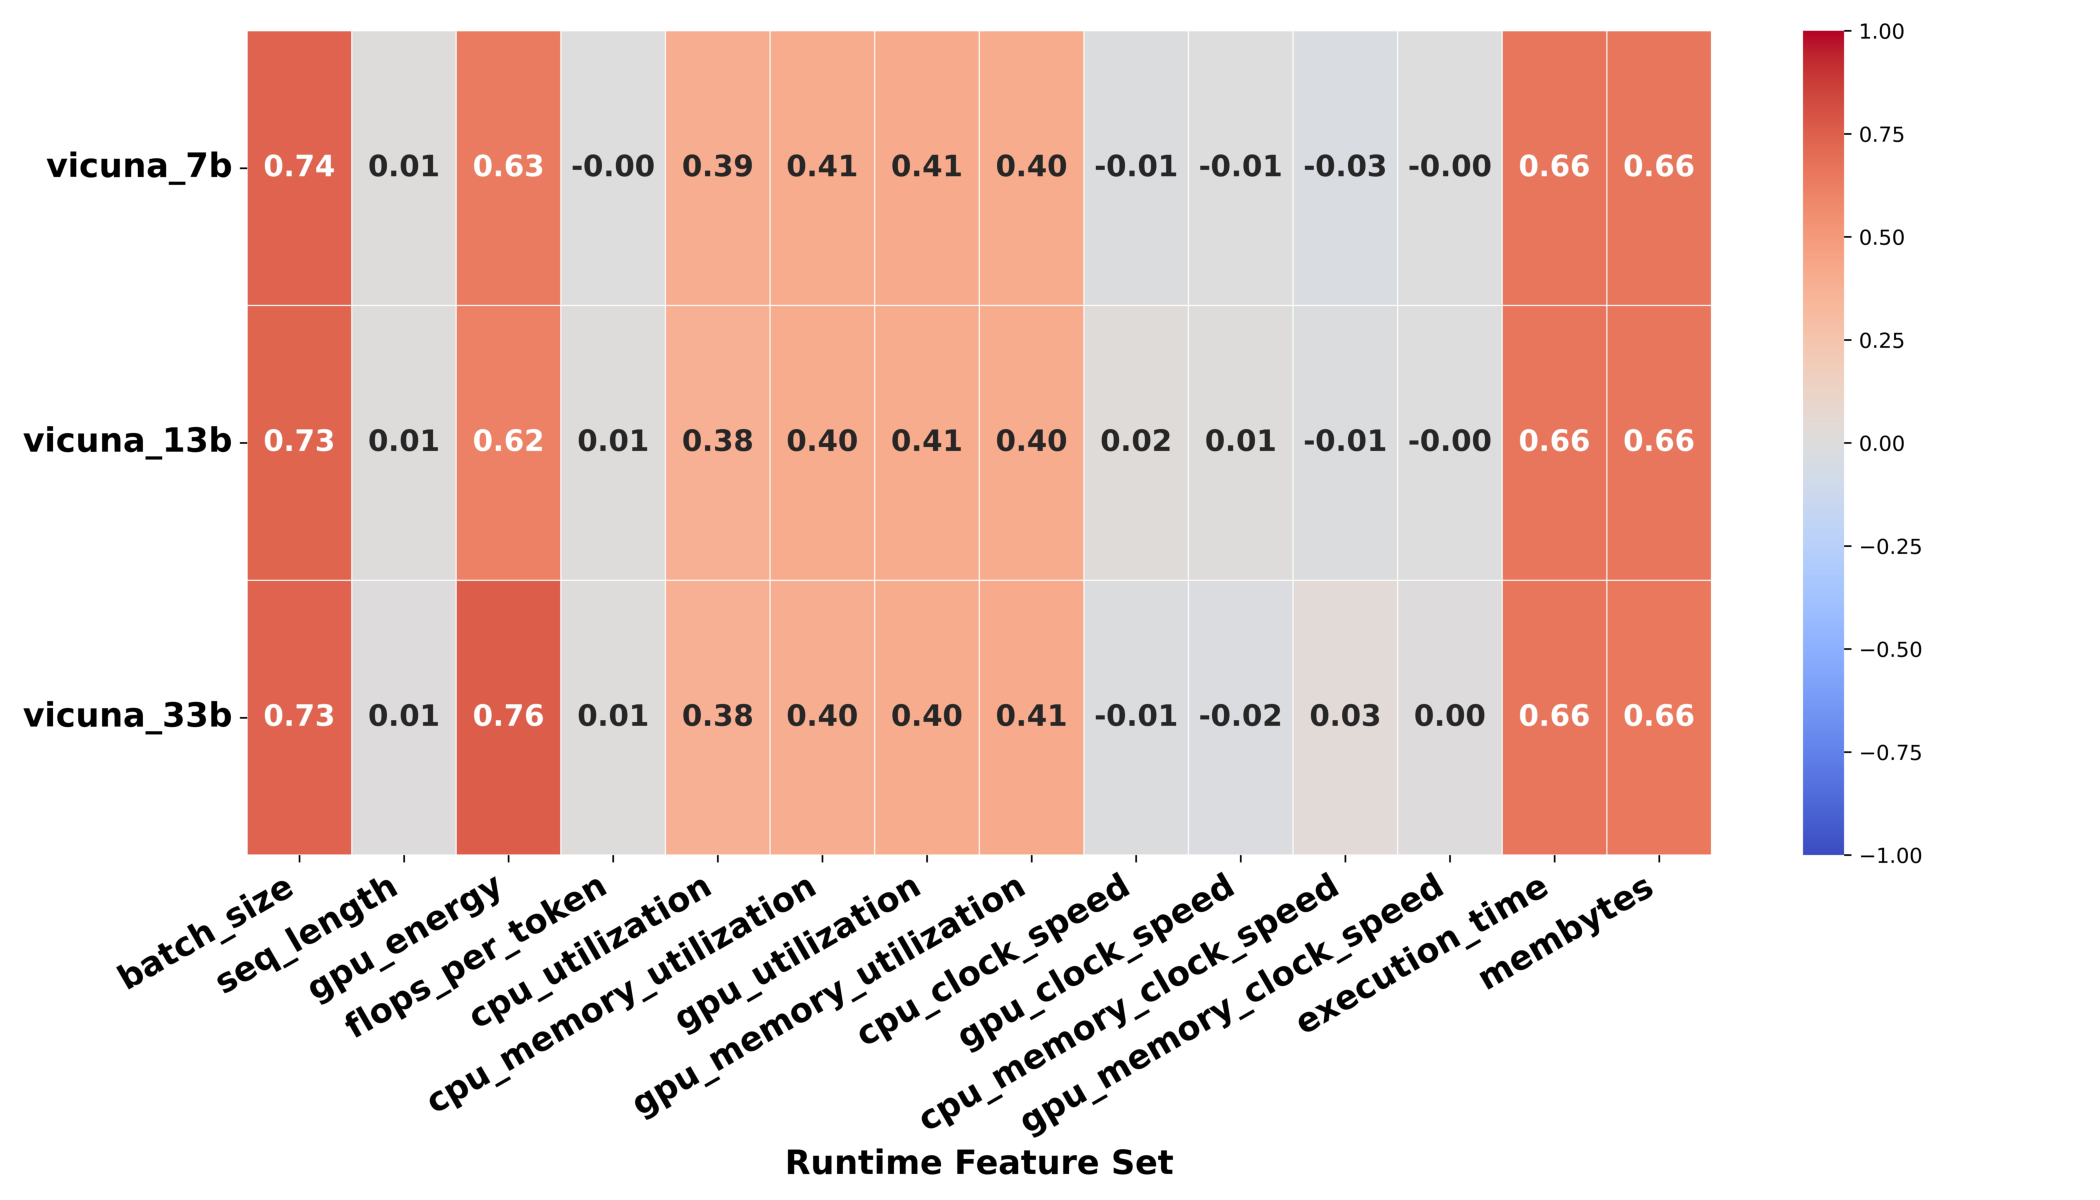
\includegraphics[width=\columnwidth]{figures/vicuna_energy_correlations_4GPU.pdf}
% \caption{Spearman correlation heatmap of runtime features for the Total Model Energy of the 3 Vicuna models with the runtime features.}
% \label{fig:correlation_heatmap}
% % \vspace{-6pt}
% \end{figure}



To assess the influence of different input features on total energy consumption, we performed a Spearman rank correlation analysis across all model configurations for Vicuna. %As shown in Figure~\ref{fig:correlation_heatmap}, GPU energy reported by NVML exhibits a strong correlation with total energy ($\rho$ between $0.633$ and $0.762$), as expected since GPU computation dominates energy consumption in LLMs. 

GPU energy reported by NVML exhibits a strong correlation with total energy ($\rho$ between $0.633$ and $0.762$), as expected since GPU computation dominates energy consumption in LLMs. 
However, other features also show substantial correlations with total energy consumption. Runtime features are particularly strongly correlated with total energy, with batch size ($\rho$ between $0.735$ and $0.737$), execution time ($\rho$ between $0.658$ and $0.664$), and Memory ($\rho$ between $0.656$ and $0.663$) all showing strong correlations. 

These results further demonstrate that apart from GPU energy other system-level utilization metrics also capture critical aspects of energy consumption - particularly in tensor-parallel configurations where communication and synchronization overheads are significant. 



% \section{Ground Truth Energy vs Inference Time plot}
% \label{app:ground-truth-energy}

% \begin{figure}[!t]
% \centering
% % 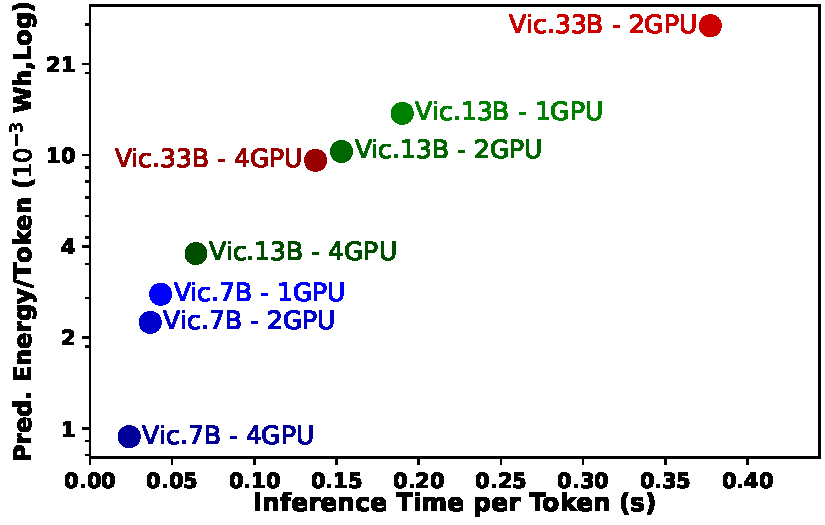
\includegraphics[width=\columnwidth]{figures/pareto_plot.pdf}

% \caption{Actual energy per token vs. inference time per token (log scale) for Vicuna models.\anshul{use wrapfig here too, such a big figure looks bad. make y-axis range same as use case figure else it seems our predictions are significantly off.}}
% \label{fig:pareto_plot_ground_truth}
% % \vspace{-6pt}
% \end{figure}

% Figure~\ref{fig:pareto_plot_ground_truth} shows the trade-off between actual energy consumption and inference time per token across Vicuna model sizes and GPU configurations.
% This is discussed in the context of generalization within the optimal model selection use case in Section~\ref{sec:usecase}.



% \section{Ablation: Role of Model Features}
% \label{app:ablation}

% To assess the contribution of model structure features (e.g. attention heads, feed-forward dimension etc.), we perform an ablation by removing them from the prediction model and comparing MAPE with and without these features for all the variants of Vicuna.
% \begin{table}[t]
% \centering
% \small
% \setlength{\tabcolsep}{4pt}
% \renewcommand{\arraystretch}{1.05}

% \begin{tabular}{
%   @{}
%   l
%   c
%   c
%   @{}
% }
% \toprule
% \textbf{Model} & \textbf{With Model} & \textbf{Without Model} \\
% \textbf{Variant} & \textbf{Features} & \textbf{Features} \\
% \midrule
% \rowcolor{rowblue} Vicuna 7B  & 15.84\% & 17.2\% \\
% Vicuna 13B                    & 17.72\% & 18.2\% \\
% \rowcolor{rowblue} Vicuna 33B & 17.55\% & 20.1\% \\
% \bottomrule
% \end{tabular}

% \caption{Leave-one-out model-level prediction MAPE on NVIDIA A6000 GPUs with and without model features.}
% \label{tab:ablation_model_features}
% \end{table}





% As shown in Table~\ref{tab:ablation_model_features}, while overall prediction accuracy remains similar in full-data settings,
% the inclusion of model features improves generalization performance in leave-one-out evaluations—reducing MAPE by 2–4\% across Vicuna variants. These results suggest that model features help the regressors capture structural differences between variants, improving robustness when extrapolating to unseen configurations. Although the effect on raw prediction accuracy is modest, the improvement in generalization justifies their inclusion in the final model.

\section{Additional Results: Using Latency Prediction Approaches to Predict Energy}
\label{app:latency-ablation}
We evaluate whether a latency-prediction-style approach can be repurposed for energy prediction. 
Specifically, we implement a NeuSight-style baseline for energy prediction~\cite{neusight}. 
NeuSight is a recent latency-prediction framework that decomposes model execution into fine-grained matrix tiles, extracts computational features such as FLOPs and memory behavior, and trains a Multi-Layer Perceptron (MLP) to predict latency. 
We keep the same decomposition and prediction structure, but replace the prediction target with measured system energy. 
This directly tests whether latency-oriented execution features are sufficient for energy prediction.

\begin{table}[t]
\centering
\small
\setlength{\tabcolsep}{6pt}
\renewcommand{\arraystretch}{1.05}

\begin{tabular}{l|c}
\hline
\textbf{Model} & \textbf{MAPE} \tabularnewline
\hline
\rowcolor{rowblue} Vicuna 7B  & 79.19\% \tabularnewline
Vicuna 13B                    & 93.24\% \tabularnewline
\rowcolor{rowblue} Vicuna 33B & 89.38\% \tabularnewline
\hline
\end{tabular}
\vspace{-6pt}
\caption{MAPE for a NeuSight-style latency prediction framework when energy is used as the prediction target.}
\vspace{-6pt}
\label{tab:neusight_energy_target}
\end{table}

Table~\ref{tab:neusight_energy_target} shows that directly substituting energy as the prediction target performs poorly, with an average MAPE of 87.3\%. 
This corresponds to roughly $\sim$3-5$\times$ worse prediction accuracy than \sys{} and $\sim$1-2$\times$ worse accuracy than the least accurate energy-prediction baseline in our evaluation. 
This result shows that energy prediction is not simply latency prediction with a different target label. 
Latency-oriented features capture how long kernels execute, but they do not sufficiently capture the power dynamics, communication overheads, and synchronization effects that determine total system energy during parallel inference.

% \subsubsection{Extending latency prediction techniques to energy}
% %
% \aruna{can be removed, content is moved to main text}
% To demonstrate that latency prediction is not directly analogous to energy prediction, we extend the NeuSight work~\cite{neusight} by a one-to-one substitution of the prediction target  from latency to energy. 
% We choose NeuSight because it is a recent (2025) latency prediction framework that, like \sys{}, decomposes model execution (into fine-grained matrix tiles) and re-composes them to predict end-to-end performance.
% NeuSight captures computational metrics such as FLOPs and memory during execution, and trains a Multi-Layer Perceptron (MLP) to predict latency.
% %\arunacomment{Add something about why you chouse Neusight. May be this is more recent work?}  
% We capture ground truth energy during execution to train the MLP and predict the energy of an unseen test set using the same framework. 

% Our results in Table~\ref{tab:tiling_analogous_4gpu} show that a direct substitution of the prediction target in NeuSight from latency to energy leads to $\sim$3-5$\times$ worse prediction accuracy compared to \sys{} and $\sim$1-2$\times$ worse accuracy compared to the least accurate energy prediction baseline we tested. 



% \begin{table}[t]
% \centering
% \small
% \setlength{\tabcolsep}{6pt}
% \renewcommand{\arraystretch}{1.1}

% \begin{tabular}{l|c}
% \hline
% \textbf{Model} & \textbf{MAPE} \\
% \hline
% \rowcolor{rowblue} Vicuna 7B  & 79.19\% \\
% Vicuna 13B                   & 93.24\% \\
% \rowcolor{rowblue} Vicuna 33B & 89.38\% \\
% \hline
% \end{tabular}

% \caption{MAPE results for NeuSight~\cite{neusight} based prediction with energy as the predictor target.}
% \label{tab:tiling_analogous_4gpu}
% \end{table}


\begin{table}[t]
\centering
\small
\setlength{\tabcolsep}{5pt}
\renewcommand{\arraystretch}{1.05}

\begin{tabular}{lclc}
\toprule
\textbf{Model} & \textbf{MAPE} & \textbf{Model} & \textbf{MAPE} \tabularnewline
\midrule
\rowcolor{rowblue} Vicuna 7B  & 13.34\% & Llama 7B  & 15.30\% \tabularnewline
Vicuna 13B                    & 13.78\% & Llama 13B & 16.51\% \tabularnewline
\rowcolor{rowblue} Vicuna 33B & 14.45\% & Llama 70B & 26.53\% \tabularnewline
Mistral 8B                    & 16.25\% & Qwen 8B   & 16.07\% \tabularnewline
\rowcolor{rowblue} Mistral 24B & 17.25\% & Qwen 14B  & 19.41\% \tabularnewline
Mistral 48B                   & 17.83\% & Qwen 32B  & 14.90\% \tabularnewline
\bottomrule
\end{tabular}

\vspace{-6pt}
\caption{Model-level prediction results for \sys{} on 2$\times$ NVIDIA H200 GPUs.}
\label{tab:h200_model_results}
\vspace{-6pt}
\end{table}


\section{Additional Results on NVIDIA H200 GPUs}
\label{app:additional_perf_results}

Table~\ref{tab:h200_model_results} reports additional model-level prediction results for \sys{} on NVIDIA H200 GPUs. 
These results correspond to the H200 hardware-extension experiment referenced in \S\ref{sec:model_prediction}. 
Across the evaluated model variants, \sys{} achieves an average MAPE of 16.8\%, showing that the same model-tree decomposition and communication- prediction methodology remain effective on a H200s as well.


Table~\ref{tab:h200_module_results} reports module-level prediction results for \sys{} on H200. 
The prediction error remains in the single-digit range across the evaluated modules, including the communication-heavy AllReduce module.

% \vspace{-6pt}

These results provide additional evidence that \sys{} is not tied to a single GPU platform. 
The H200 experiments show that the same decomposition, communication modeling, and structural/runtime feature set can be reused on an additional GPU platform with modest prediction error.

\begin{table}[H]
\centering
\small
\setlength{\tabcolsep}{6pt}
\renewcommand{\arraystretch}{1.05}

\begin{tabular}{lc}
\toprule
\textbf{Module} & \textbf{H200 MAPE} \tabularnewline
\midrule
\rowcolor{rowblue} Self-Attention      & 8.80\% \tabularnewline
MLP                                    & 7.44\% \tabularnewline
\rowcolor{rowblue} AllReduce           & 9.25\% \tabularnewline
LayerNorm/RMSNorm                      & 8.12\% \tabularnewline
\rowcolor{rowblue} LLMEmbedding        & 7.78\% \tabularnewline
\bottomrule
\end{tabular}

\vspace{-6pt}
\caption{Module-level MAPE for \sys{} on NVIDIA H200 GPUs.}
\label{tab:h200_module_results}
\vspace{-6pt}
\end{table}

% \section{Additional Results on NVIDIA B40 and H100 GPUs}
% \label{app:additional_perf_results}

% {To further evaluate whether PIE-P remains effective beyond the primary GPU platform used in our main experiments, we extend our evaluation to two additional GPU platforms: NVIDIA~B40 and NVIDIA~H100. These experiments serve as hardware-extension studies, showing that PIE-P's module-level decomposition and feature-based prediction remain accurate when the underlying GPU architecture and runtime behavior change.}

% {The B40 results show that PIE-P continues to provide accurate fine-grained energy estimates across the major modules of transformer inference. At the module level, PIE-P achieves single-digit MAPE across the main compute and communication components: 7.8\% for Self-Attention, 6.6\% for MLP, 8.2\% for AllReduce, 7.2\% for LayerNorm, and 6.9\% for Embedding. These results show that the predictor is not only fitting end-to-end model energy, but also preserving accuracy at the level of the individual modules used by the model-tree abstraction. In particular, the low AllReduce error on B40 indicates that the communication-aware component of PIE-P remains effective under a different GPU platform.}

% % {We also evaluate leave-one-out generalization on B40 in the 2-GPU setting across multiple model families. For Vicuna, the held-out model errors are 11.83\%, 12.22\%, and 12.81\% for the 7B, 13B, and 33B variants, respectively. Mistral shows slightly higher but still moderate errors of 14.41\%, 15.29\%, and 15.81\% across its variants. Llama shows 13.56\% and 14.64\% for the 7B and 13B models, while the larger 70B model is more challenging at 23.52\%. Qwen achieves 14.25\%, 17.21\%, and 13.21\% across its 8B, 14B, and 32B variants.}

% \aruna{Please add a table for H100 results, no need for leave-one-out I think. }
% {For the 2-GPU H100 setting, PIE-P shows a modest increase in prediction error relative to B40, with each corresponding MAPE value increased by 12.8\%. At the module level, PIE-P obtains 8.80\% for Self-Attention, 7.44\% for MLP, 9.25\% for AllReduce, 8.12\% for LayerNorm, and 7.78\% for Embedding. Despite the increase, the module-level errors remain in the single-digit range, indicating that the same communication-aware decomposition continues to capture the major sources of energy consumption on H100.}

% {The leave-one-out results on H100 also remain moderate in the 2-GPU setting. For Vicuna, the held-out model errors are 13.34\%, 13.78\%, and 14.45\% for the 7B, 13B, and 33B variants, respectively. Mistral obtains 16.25\%, 17.25\%, and 17.83\% across its variants. Llama obtains 15.30\% and 16.51\% for the 7B and 13B models, while the larger 70B model reaches 26.53\%. Qwen obtains 16.07\%, 19.41\%, and 14.90\% across its 8B, 14B, and 32B variants. These results suggest that while H100 introduces somewhat higher prediction error, PIE-P's feature-based and communication-aware design remains effective across GPU platforms.}

% {For the 4-GPU B40 setting, PIE-P again maintains reasonable accuracy across families. Vicuna obtains 14.21\%, 13.39\%, and 15.25\% MAPE across the 7B, 13B, and 33B variants. Mistral obtains 16.66\%, 19.29\%, and 19.71\%, while Qwen obtains 14.54\%, 16.34\%, and 14.91\%. Taken together, these results provide additional evidence that PIE-P is not tied to a single GPU platform. Although a fully hardware-agnostic predictor remains future work, the B40 and H100 experiments show that the same decomposition, communication modeling, and structural/runtime feature set can be reused successfully on additional GPU platforms with modest prediction error.}






% Requires the same packages/macros as the existing appendix tables:
% \usepackage{booktabs}
% \usepackage[table]{xcolor}
% \usepackage{array}
% and an existing rowblue definition.


% \begin{table}[t]
% \centering
% \small
% \setlength{\tabcolsep}{3pt}
% \renewcommand{\arraystretch}{1.05}

% \begin{tabular}{
% @{}
% l
% c
% l
% c
% @{}
% }
% \toprule
% \textbf{Model} & \textbf{MAPE} & \textbf{Model} & \textbf{MAPE} \\
% \midrule
% \rowcolor{rowblue} Vicuna 7B   & 41.1\% & Llama 7B   & 53.1\%  \\
% Vicuna 13B                     & 48.3\% & Llama 13B  & 51.2\%  \\
% \rowcolor{rowblue} Vicuna 33B  & 52.8\% & Llama 70B  & 112.5\% \\
% \midrule
% Mistral 8B                     & 41.2\% & Qwen 8B    & 38.4\%  \\
% \rowcolor{rowblue} Mistral 24B & 43.4\% & Qwen 14B   & 39.9\%  \\
% Mistral 48B                    & 43.8\% & Qwen 32B   & 41.1\%  \\
% \bottomrule
% \end{tabular}

% \caption{MAPE when using NVML-reported GPU energy as a proxy for total system energy on NVIDIA B40 GPUs. This approach produces substantially higher errors compared to \sys{}.}
% \label{tab:b40_nvml_proxy}
% \end{table}


% \begin{table}[t]
% \centering
% \small
% \setlength{\tabcolsep}{3pt}
% \renewcommand{\arraystretch}{1.05}

% \begin{tabular}{
% @{}
% l
% c
% l
% c
% @{}
% }
% \toprule
% \textbf{Model} & \textbf{MAPE} & \textbf{Model} & \textbf{MAPE} \\
% \midrule
% \rowcolor{rowblue} Vicuna 7B   & 63.6\% & Llama 7B   & 71.4\%  \\
% Vicuna 13B                     & 62.3\% & Llama 13B  & 79.3\%  \\
% \rowcolor{rowblue} Vicuna 33B  & 68.9\% & Llama 70B  & 115.2\% \\
% \midrule
% Mistral 8B                     & 48.3\% & Qwen 8B    & 63.1\%  \\
% \rowcolor{rowblue} Mistral 24B & 61.2\% & Qwen 14B   & 68.2\%  \\
% Mistral 48B                    & 61.9\% & Qwen 32B   & 65.5\%  \\
% \bottomrule
% \end{tabular}

% \caption{Leave-one-out generalization results for NVML-based regression on NVIDIA B40 GPUs. Each row shows MAPE when using NVML measurements to predict total energy for a model excluded from training.}
% \label{tab:b40_nvml_loo}
% \end{table}



% \anurag{ablation for methodology - maybe predict directly the  model energy}
% \anurag{ablation for communication modelling methodology}
% \anurag{tables for h100 results}
% \anurag{additional writeup for the B40 results in the main result/evaluation section}


\end{document}